\documentclass[10pt]{beamer} % aspect ratio 4:3, 128 mm by 96 mm
%\documentclass[10pt,aspectratio=169]{beamer} % aspect ratio 16:9
%\graphicspath{{../../figures/}}
\graphicspath{{figs/}{../../figures/}{../../journal_papers/Composite_Structures_GA/figs/}}
%\includeonlyframes{frame1,frame2,frame3,frame4,frame5,frame6,frame7,frame8,frame9}
%\includeonlyframes{frame10,frame11,frame12,frame13}
%\includeonlyframes{frame14,frame15,frame16,frame17,frame18,frame19,frame20,frame21}
%\includeonlyframes{frame22,frame23,frame24,frame25,frame26}
%\includeonlyframes{frame27,frame28}
%%%%%%%%%%%%%%%%%%%%%%%%%%%%%%%%%%%%%%%%%%%%%%%%%%
% Packages
%%%%%%%%%%%%%%%%%%%%%%%%%%%%%%%%%%%%%%%%%%%%%%%%%%
\usepackage{appendixnumberbeamer}
\usepackage{booktabs}
\usepackage{csvsimple} % for csv read
\usepackage[scale=2]{ccicons}
\usepackage{pgfplots}
\usepackage{xspace}
\usepackage{amsmath}
\usepackage{totcount}
\usepackage{tikz}
%\usepackage{comment}
%\usetikzlibrary{external} % speedup compilation
%\tikzexternalize % activate!
%\usetikzlibrary{shapes,arrows}  

%\usepackage{bibentry}
%\nobibliography*
\usepackage{caption}%
\captionsetup[figure]{labelformat=empty}%
%%%%%%%%%%%%%%%%%%%%%%%%%%%%%%%%%%%%%%%%%%%%%%%%%%
% Metropolis theme custom modification file
%%%%%%%%%%%%%%%%%%%%%%%%%%%%%%%%%%%%%%%%%%%%%%%%%%
% Metropolis theme custom modification file
%%%%%%%%%%%%%%%%%%%%%%%%%%%%%%%%%%%%%%%%%%%%%%%%%%
% Metropolis theme custom colors
%%%%%%%%%%%%%%%%%%%%%%%%%%%%%%%%%%%%%%%%%%%%%%%%%%
\usetheme[progressbar=foot]{metropolis}
\useoutertheme{metropolis}
\useinnertheme{metropolis}
\usefonttheme{metropolis}
\setbeamercolor{background canvas}{bg=white}

%\usecolortheme{spruce}

\definecolor{myblue}{rgb}{0.19,0.55,0.91}
\definecolor{mediumblue}{rgb}{0,0,205}
\definecolor{darkblue}{rgb}{0,0,139}
\definecolor{Dodgerblue}{HTML}{1E90FF}
\definecolor{Navy}{HTML}{000080} % {rgb}{0,0,128}
\definecolor{Aliceblue}{HTML}{F0F8FF}
\definecolor{Lightskyblue}{HTML}{87CEFA}
\definecolor{logoblue}{RGB}{1,67,140}
\definecolor{Purple}{HTML}{911146}
\definecolor{Orange}{HTML}{CF4A30}

\setbeamercolor{progress bar}{bg=Lightskyblue}
\setbeamercolor{progress bar}{ fg=logoblue} 
\setbeamercolor{frametitle}{bg=logoblue}
\setbeamercolor{title separator}{fg=logoblue}
\setbeamercolor{block title}{bg=Lightskyblue!30,fg=black}
\setbeamercolor{block body}{bg=Lightskyblue!15,fg=black}
\setbeamercolor{alerted text}{fg=Purple}
%%%%%%%%%%%%%%%%%%%%%%%%%%%%%%%%%%%%%%%%%%%%%%%%%%
%  Theme modifications
%%%%%%%%%%%%%%%%%%%%%%%%%%%%%%%%%%%%%%%%%%%%%%%%%%
% modify progress bar linewidth
\makeatletter
\setlength{\metropolis@progressinheadfoot@linewidth}{2pt} 
\setlength{\metropolis@titleseparator@linewidth}{1pt}
\setlength{\metropolis@progressonsectionpage@linewidth}{1pt}

\setbeamertemplate{progress bar in section page}{
	\setlength{\metropolis@progressonsectionpage}{%
		\textwidth * \ratio{\thesection pt}{\totvalue{totalsection} pt}%
	}%
	\begin{tikzpicture}
	\fill[bg] (0,0) rectangle (\textwidth, \metropolis@progressonsectionpage@linewidth);
	\fill[fg] (0,0) rectangle (\metropolis@progressonsectionpage, \metropolis@progressonsectionpage@linewidth);
	\end{tikzpicture}%
}
\makeatother
\newcounter{totalsection}
\regtotcounter{totalsection}

\AtBeginDocument{%
	\pretocmd{\section}{\refstepcounter{totalsection}}{\typeout{Yes, prepending was successful}}{\typeout{No, prepending was not successful}}%
}%
%%%%%%%%%%%%%%%%%%%%%%%%%%%%%%%%%%%%%%%%%%%%%%%%%%
%  Bibliography mods
%%%%%%%%%%%%%%%%%%%%%%%%%%%%%%%%%%%%%%%%%%%%%%%%%%
\setbeamertemplate{bibliography item}{\insertbiblabel} %% Remove book symbol from references and add number in square brackets
% kill the abominable icon (without number)
%\setbeamertemplate{bibliography item}{}
%\makeatletter
%\renewcommand\@biblabel[1]{#1.} % number only
%\makeatother
% remove line breaks in bibliography
\setbeamertemplate{bibliography entry title}{}
\setbeamertemplate{bibliography entry location}{}
%%%%%%%%%%%%%%%%%%%%%%%%%%%%%%%%%%%%%%%%%%%%%%%%%%
%  Bibliography custom commands
%%%%%%%%%%%%%%%%%%%%%%%%%%%%%%%%%%%%%%%%%%%%%%%%%%
\newcommand{\bibliotitlestyle}[1]{\textbf{#1}\par}

\newif\ifinbiblio
\newcounter{bibkey}
\newenvironment{biblio}[2][long]{%
    %\setbeamertemplate{bibliography item}{\insertbiblabel}
    \setbeamertemplate{bibliography item}{}% without numbers
	\setbeamerfont{bibliography item}{size=\footnotesize}
	\setbeamerfont{bibliography entry author}{size=\footnotesize}
	\setbeamerfont{bibliography entry title}{size=\footnotesize}
	\setbeamerfont{bibliography entry location}{size=\footnotesize}
	\setbeamerfont{bibliography entry note}{size=\footnotesize}
	\ifx!#2!\else%
	\bibliotitlestyle{#2}%
	\fi%
	\begin{thebibliography}{}%
		\inbibliotrue%
		\setbeamertemplate{bibliography entry title}[#1]%
	}{%
		\inbibliofalse%
		\setbeamertemplate{bibliography item}{}%
	\end{thebibliography}%
}

\newcommand{\biblioref}[5][short]{
	\setbeamertemplate{bibliography entry title}[#1]
	\stepcounter{bibkey}%
	\ifinbiblio%
	\bibitem{\thebibkey}%
	#2
	\newblock #4
	\ifx!#5!\else\newblock {\em #5}, #3 \fi%
	\else%
	\begin{biblio}{}
		\bibitem{\thebibkey}
		#2
		\newblock #4
		\ifx!#5!\else\newblock {\em #5}, #3\fi
	\end{biblio}
	\fi
}
%
%\newbibmacro*{hypercite}{%
%	\renewcommand{\@makefntext}[1]{\noindent\normalfont##1}%
%	\footnotetext{%
%		\blxmkbibnote{foot}{%
%			\printtext[labelnumberwidth]{%
%				\printfield{prefixnumber}%
%				\printfield{labelnumber}}%
%			\addspace
%			\fullcite{\thefield{entrykey}}}}}
%
%\DeclareCiteCommand{\hypercite}%
%{\usebibmacro{cite:init}}
%{\usebibmacro{hypercite}}
%{}
%{\usebibmacro{cite:dump}}
%
%% Redefine the \footfullcite command to use the reference number
%\renewcommand{\footfullcite}[1]{\cite{#1}\hypercite{#1}}
%%%%%%%%%%%%%%%%%%%%%%%%%%%%%%%%%%%%%%%%%%%%%%%%%%
% Custom commands
%%%%%%%%%%%%%%%%%%%%%%%%%%%%%%%%%%%%%%%%%%%%%%%%%%
% matrix command 
\newcommand{\matr}[1]{\mathbf{#1}} % bold upright (Elsevier, Springer)
%\newcommand{\matr}[1]{#1}          % pure math version
%\newcommand{\matr}[1]{\bm{#1}}     % ISO complying version
% vector command 
\newcommand{\vect}[1]{\mathbf{#1}} % bold upright (Elsevier, Springer)
% bold symbol
\newcommand{\bs}[1]{\boldsymbol{#1}}
% derivative upright command
\DeclareRobustCommand*{\drv}{\mathop{}\!\mathrm{d}}
\newcommand{\ud}{\mathrm{d}}
% 
\newcommand{\themename}{\textbf{\textsc{metropolis}}\xspace}

%%%%%%%%%%%%%%%%%%%%%%%%%%%%%%%%%%%%%%%%%%%%%%%%%%
%  Title page options
%%%%%%%%%%%%%%%%%%%%%%%%%%%%%%%%%%%%%%%%%%%%%%%%%%
% \date{\today}
\date{}
%%%%%%%%%%%%%%%%%%%%%%%%%%%%%%%%%%%%%%%%%%%%%%%%%%
% option 1
%%%%%%%%%%%%%%%%%%%%%%%%%%%%%%%%%%%%%%%%%%%%%%%%%%
\title{Elastic constants identification of composite laminates by using Lamb wave dispersion curves and optimization methods}
\subtitle{Lamb-opt}
\author{\textbf{Paweł Kudela}\\Maciej Radzieński \\Piotr Fiborek\\Tomasz Wandowski }
% logo align to Institute 
\institute{Institute of Fluid Flow Machinery\\Polish Academy of Sciences \\ \vspace{-1.5cm}\flushright 
\includegraphics[width=4cm]{../images/logo/logo_eng_40mm.eps}}
%%%%%%%%%%%%%%%%%%%%%%%%%%%%%%%%%%%%%%%%%%%%%%%%%%
% option 2 - authors in one line
%%%%%%%%%%%%%%%%%%%%%%%%%%%%%%%%%%%%%%%%%%%%%%%%%%
%	\title{Elastic constants identification of composite laminates by using Lamb wave dispersion curves and optimization methods}
%	\subtitle{Lamb-opt}
%	\author{\textbf{Paweł Kudela}\textsuperscript{2}, Maciej Radzieński\textsuperscript{2}, Wiesław Ostachowicz\textsuperscript{2}, Zhibo Yang\textsuperscript{1} }
%	% logo align to Institute 
%	\institute{\textsuperscript{1}Xi'an Jiaotong University \\ \textsuperscript{2}Institute of Fluid Flow Machinery\\ \hspace*{1pt} Polish Academy of Sciences \\ \vspace{-1.5cm}\flushright 
\includegraphics[width=4cm]{../images/logo/logo_eng_40mm.eps}}
%%%%%%%%%%%%%%%%%%%%%%%%%%%%%%%%%%%%%%%%%%%%%%%%%%
% option 3 - multilogo vertical
%%%%%%%%%%%%%%%%%%%%%%%%%%%%%%%%%%%%%%%%%%%%%%%%%%
%\title{Elastic constants identification of composite laminates by using Lamb wave dispersion curves and optimization methods}
%\subtitle{Lamb-opt}
%	\author{\textbf{Paweł Kudela}\inst{1}, Maciej Radzieński\inst{1}, Wiesław Ostachowicz\inst{1}, Zhibo Yang\inst{2} }
%	% logo under Institute 
%	\institute%
%	{ 
%		\inst{1}%
%		Institute of Fluid Flow Machinery\\ \hspace*{1pt} Polish Academy of Sciences \\ 
\includegraphics[height=0.85cm]{../images/logo/logo_eng_40mm.eps} \\
%		\and
%		\inst{2}%
%	    Xi'an Jiaotong University \\ 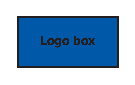
\includegraphics[height=0.85cm]{../images/logo/logo_box.eps}
%    }
% end od option 3
%%%%%%%%%%%%%%%%%%%%%%%%%%%%%%%%%%%%%%%%%%%%%%%%%%
%% option 4 - 3 Institutes and logos horizontal centered
%%%%%%%%%%%%%%%%%%%%%%%%%%%%%%%%%%%%%%%%%%%%%%%%%%
%\title{Elastic constants identification of composite laminates by using Lamb wave dispersion curves and optimization methods}
%\subtitle{Lamb-opt }
%\author{\textbf{Paweł Kudela}\textsuperscript{1}, Maciej Radzieński\textsuperscript{1}, Marco Miniaci\textsuperscript{2}, Zhibo Yang\textsuperscript{3} }
%
%\institute{ 
%\begin{columns}[T,onlytextwidth]
%	\column{0.39\textwidth}
%	\begin{center}
%		\textsuperscript{1}Institute of Fluid Flow Machinery\\ \hspace*{3pt}Polish Academy of Sciences
%	\end{center}
%	\column{0.3\textwidth}
%	\begin{center}
%		\textsuperscript{2}Zurich University
%	\end{center}
%	\column{0.3\textwidth}
%	\begin{center}
%		\textsuperscript{3}Xi'an Jiaotong University
%	\end{center}
%\end{columns}
%\vspace{6pt}
%% logos 
%\begin{columns}[b,onlytextwidth]
%	\column{0.39\textwidth}
%		\centering 
%		
\includegraphics[width=\textwidth,height=0.85cm,keepaspectratio]{../images/logo/logo_eng_40mm.eps}
%	\column{0.3\textwidth}
%		\centering 
%		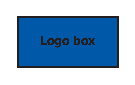
\includegraphics[width=\textwidth,height=0.85cm,keepaspectratio]{../images/logo/logo_box.eps}
%	\column{0.3\textwidth}
%		\centering 
%		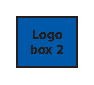
\includegraphics[width=\textwidth,height=0.85cm,keepaspectratio]{../images/logo/logo_box2.eps}
%\end{columns}
%}
%\makeatletter
%\setbeamertemplate{title page}{
%	\begin{minipage}[b][\paperheight]{\textwidth}
%		\centering  % <-- Center here
%		\ifx\inserttitlegraphic\@empty\else\usebeamertemplate*{title graphic}\fi
%		\vfill%
%		\ifx\inserttitle\@empty\else\usebeamertemplate*{title}\fi
%		\ifx\insertsubtitle\@empty\else\usebeamertemplate*{subtitle}\fi
%		\usebeamertemplate*{title separator}
%		\ifx\beamer@shortauthor\@empty\else\usebeamertemplate*{author}\fi
%		\ifx\insertdate\@empty\else\usebeamertemplate*{date}\fi
%		\ifx\insertinstitute\@empty\else\usebeamertemplate*{institute}\fi
%		\vfill
%		\vspace*{1mm}
%	\end{minipage}
%}
%
%\setbeamertemplate{title}{
%	%  \raggedright%  % <-- Comment here
%	\linespread{1.0}%
%	\inserttitle%
%	\par%
%	\vspace*{0.5em}
%}
%\setbeamertemplate{subtitle}{
%	%  \raggedright%  % <-- Comment here
%	\insertsubtitle%
%	\par%
%	\vspace*{0.5em}
%}
%\makeatother
% end of option 4
%%%%%%%%%%%%%%%%%%%%%%%%%%%%%%%%%%%%%%%%%%%%%%%%%%
% option 5 - 2 Institutes and logos horizontal centered
%%%%%%%%%%%%%%%%%%%%%%%%%%%%%%%%%%%%%%%%%%%%%%%%%%
%\title{Elastic constants identification of composite laminates by using Lamb wave dispersion curves and optimization methods}
%\subtitle{Lamb-opt }
%\author{\textbf{Paweł Kudela}\textsuperscript{1}, Maciej Radzieński\textsuperscript{1}, Marco Miniaci\textsuperscript{2}}
%
%\institute{ 
%	\begin{columns}[T,onlytextwidth]
%		\column{0.5\textwidth}
%			\centering
%			\textsuperscript{1}Institute of Fluid Flow Machinery\\ \hspace*{3pt}Polish Academy of Sciences
%		\column{0.5\textwidth}
%			\centering
%			\textsuperscript{2}Zurich University
%	\end{columns}
%	\vspace{6pt}
%	% logos 
%	\begin{columns}[b,onlytextwidth]
%		\column{0.5\textwidth}
%		\centering 
%		
\includegraphics[width=\textwidth,height=0.85cm,keepaspectratio]{../images/logo/logo_eng_40mm.eps}
%		\column{0.5\textwidth}
%		\centering 
%		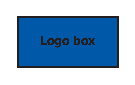
\includegraphics[width=\textwidth,height=0.85cm,keepaspectratio]{../images/logo/logo_box.eps}
%	\end{columns}
%}
%\makeatletter
%\setbeamertemplate{title page}{
%	\begin{minipage}[b][\paperheight]{\textwidth}
%		\centering  % <-- Center here
%		\ifx\inserttitlegraphic\@empty\else\usebeamertemplate*{title graphic}\fi
%		\vfill%
%		\ifx\inserttitle\@empty\else\usebeamertemplate*{title}\fi
%		\ifx\insertsubtitle\@empty\else\usebeamertemplate*{subtitle}\fi
%		\usebeamertemplate*{title separator}
%		\ifx\beamer@shortauthor\@empty\else\usebeamertemplate*{author}\fi
%		\ifx\insertdate\@empty\else\usebeamertemplate*{date}\fi
%		\ifx\insertinstitute\@empty\else\usebeamertemplate*{institute}\fi
%		\vfill
%		\vspace*{1mm}
%	\end{minipage}
%}
%
%\setbeamertemplate{title}{
%	%  \raggedright%  % <-- Comment here
%	\linespread{1.0}%
%	\inserttitle%
%	\par%
%	\vspace*{0.5em}
%}
%\setbeamertemplate{subtitle}{
%	%  \raggedright%  % <-- Comment here
%	\insertsubtitle%
%	\par%
%	\vspace*{0.5em}
%}
%\makeatother
% end of option 5
%
%%%%%%%%%%%%%%%%%%%%%%%%%%%%%%%%%%%%%%%%%%%%%%%%%%
%  End of title page options
%%%%%%%%%%%%%%%%%%%%%%%%%%%%%%%%%%%%%%%%%%%%%%%%%%
% logo option - alternative manual insertion by modification of coordinates in \put()
%\titlegraphic{%
%	%\vspace{\logoadheight}
%	\begin{picture}(0,0)
%	\put(305,-185){\makebox(0,0)[rb]{
\includegraphics[width=4cm]{../images/logo/logo_eng_40mm.eps}}}
%	\end{picture}}
%
%%%%%%%%%%%%%%%%%%%%%%%%%%%%%%%%%%%%%%%%%%%%%%%%%%
%\tikzexternalize % activate!
%%%%%%%%%%%%%%%%%%%%%%%%%%%%%%%%%%%%%%%%%%%%%%%%%%
\begin{document}
%%%%%%%%%%%%%%%%%%%%%%%%%%%%%%%%%%%%%%%%%%%%%%%%%%
\maketitle
%%%%%%%%%%%%%%%%%%%%%%%%%%%%%%%%%%%%%%%%%%%%%%%%%%
% SLIDES
%%%%%%%%%%%%%%%%%%%%%%%%%%%%%%%%%%%%%%%%%%%%%%%%%%
\begin{frame}[label=frame1]{Table of contents \label{frameone}}
  \setbeamertemplate{section in toc}[sections numbered]
  \tableofcontents[hideallsubsections]
\end{frame}
%%%%%%%%%%%%%%%%%%%%%%%%%%%%%%%%%%%%%%%%%%%%%%%%%%
\section{Introduction}
%%%%%%%%%%%%%%%%%%%%%%%%%%%%%%%%%%%%%%%%%%%%%%%%%%

%%%%%%%%%%%%%%%%%%%%%%%%%%%%%%%%%%%%%%%%%%%%%%%%%%
\begin{frame}[label=frame2]{Determination of mechanical properties of materials}
  \begin{itemize}
  	\item Destructive testing
  	\item Static tests (displacement measurements + model)
  	\item Dynamic tests (natural frequencies)
  	\item Ultrasonic methods (bulk wave velocities, ultrasonic polar scan)
  	\item \textbf{Lamb wave methods (dispersion curves)}
  \end{itemize}
\end{frame}
%%%%%%%%%%%%%%%%%%%%%%%%%%%%%%%%%%%%%%%%%%%%%%%%%%
\begin{frame}[label=frame3]{Pulsed Ultrasonic Polar Scans}
\begin{figure}
		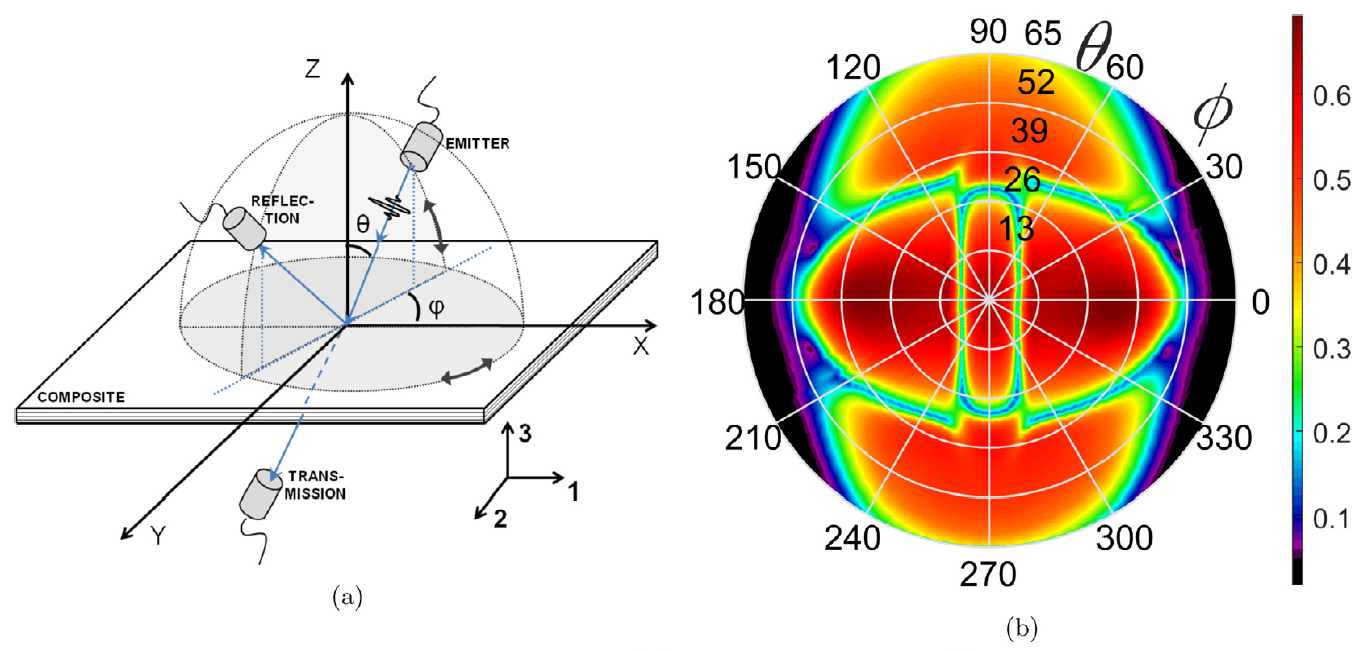
\includegraphics[width=\textwidth]{Martens-Pulsed-Ultrasonic_Polar_Scan.png}
		%\caption{ (a) Schematic of the Pulsed Ultrasonic Polar Scan (P-UPS) principle. (b) Transmission P-UPS experiment for a $[0^{\circ}]_8$ carbon/epoxy composite at 5 MHz$\cdot$ mm (amplitude).}	
\end{figure}
%Source: Martens et al.: Numerical study of the Time-of-Flight Pulsed Ultrasonic Polar Scan for the determination of the full elasticity tensor of orthotropic plates, Composite Structures 180 (2017) 29–40.
 \begin{biblio}{Source:}
	\biblioref{Martens et al.}{2017}{ Numerical study of the Time-of-Flight Pulsed Ultrasonic Polar Scan for the determination of the full elasticity tensor of orthotropic plates}{Composite Structures 180: 29–40}
\end{biblio}
\end{frame}
%%%%%%%%%%%%%%%%%%%%%%%%%%%%%%%%%%%%%%%%%%%%%%%%%%
\begin{frame}[label=frame3]{Idea of the project}
\begin{figure}
	\only<1>{
		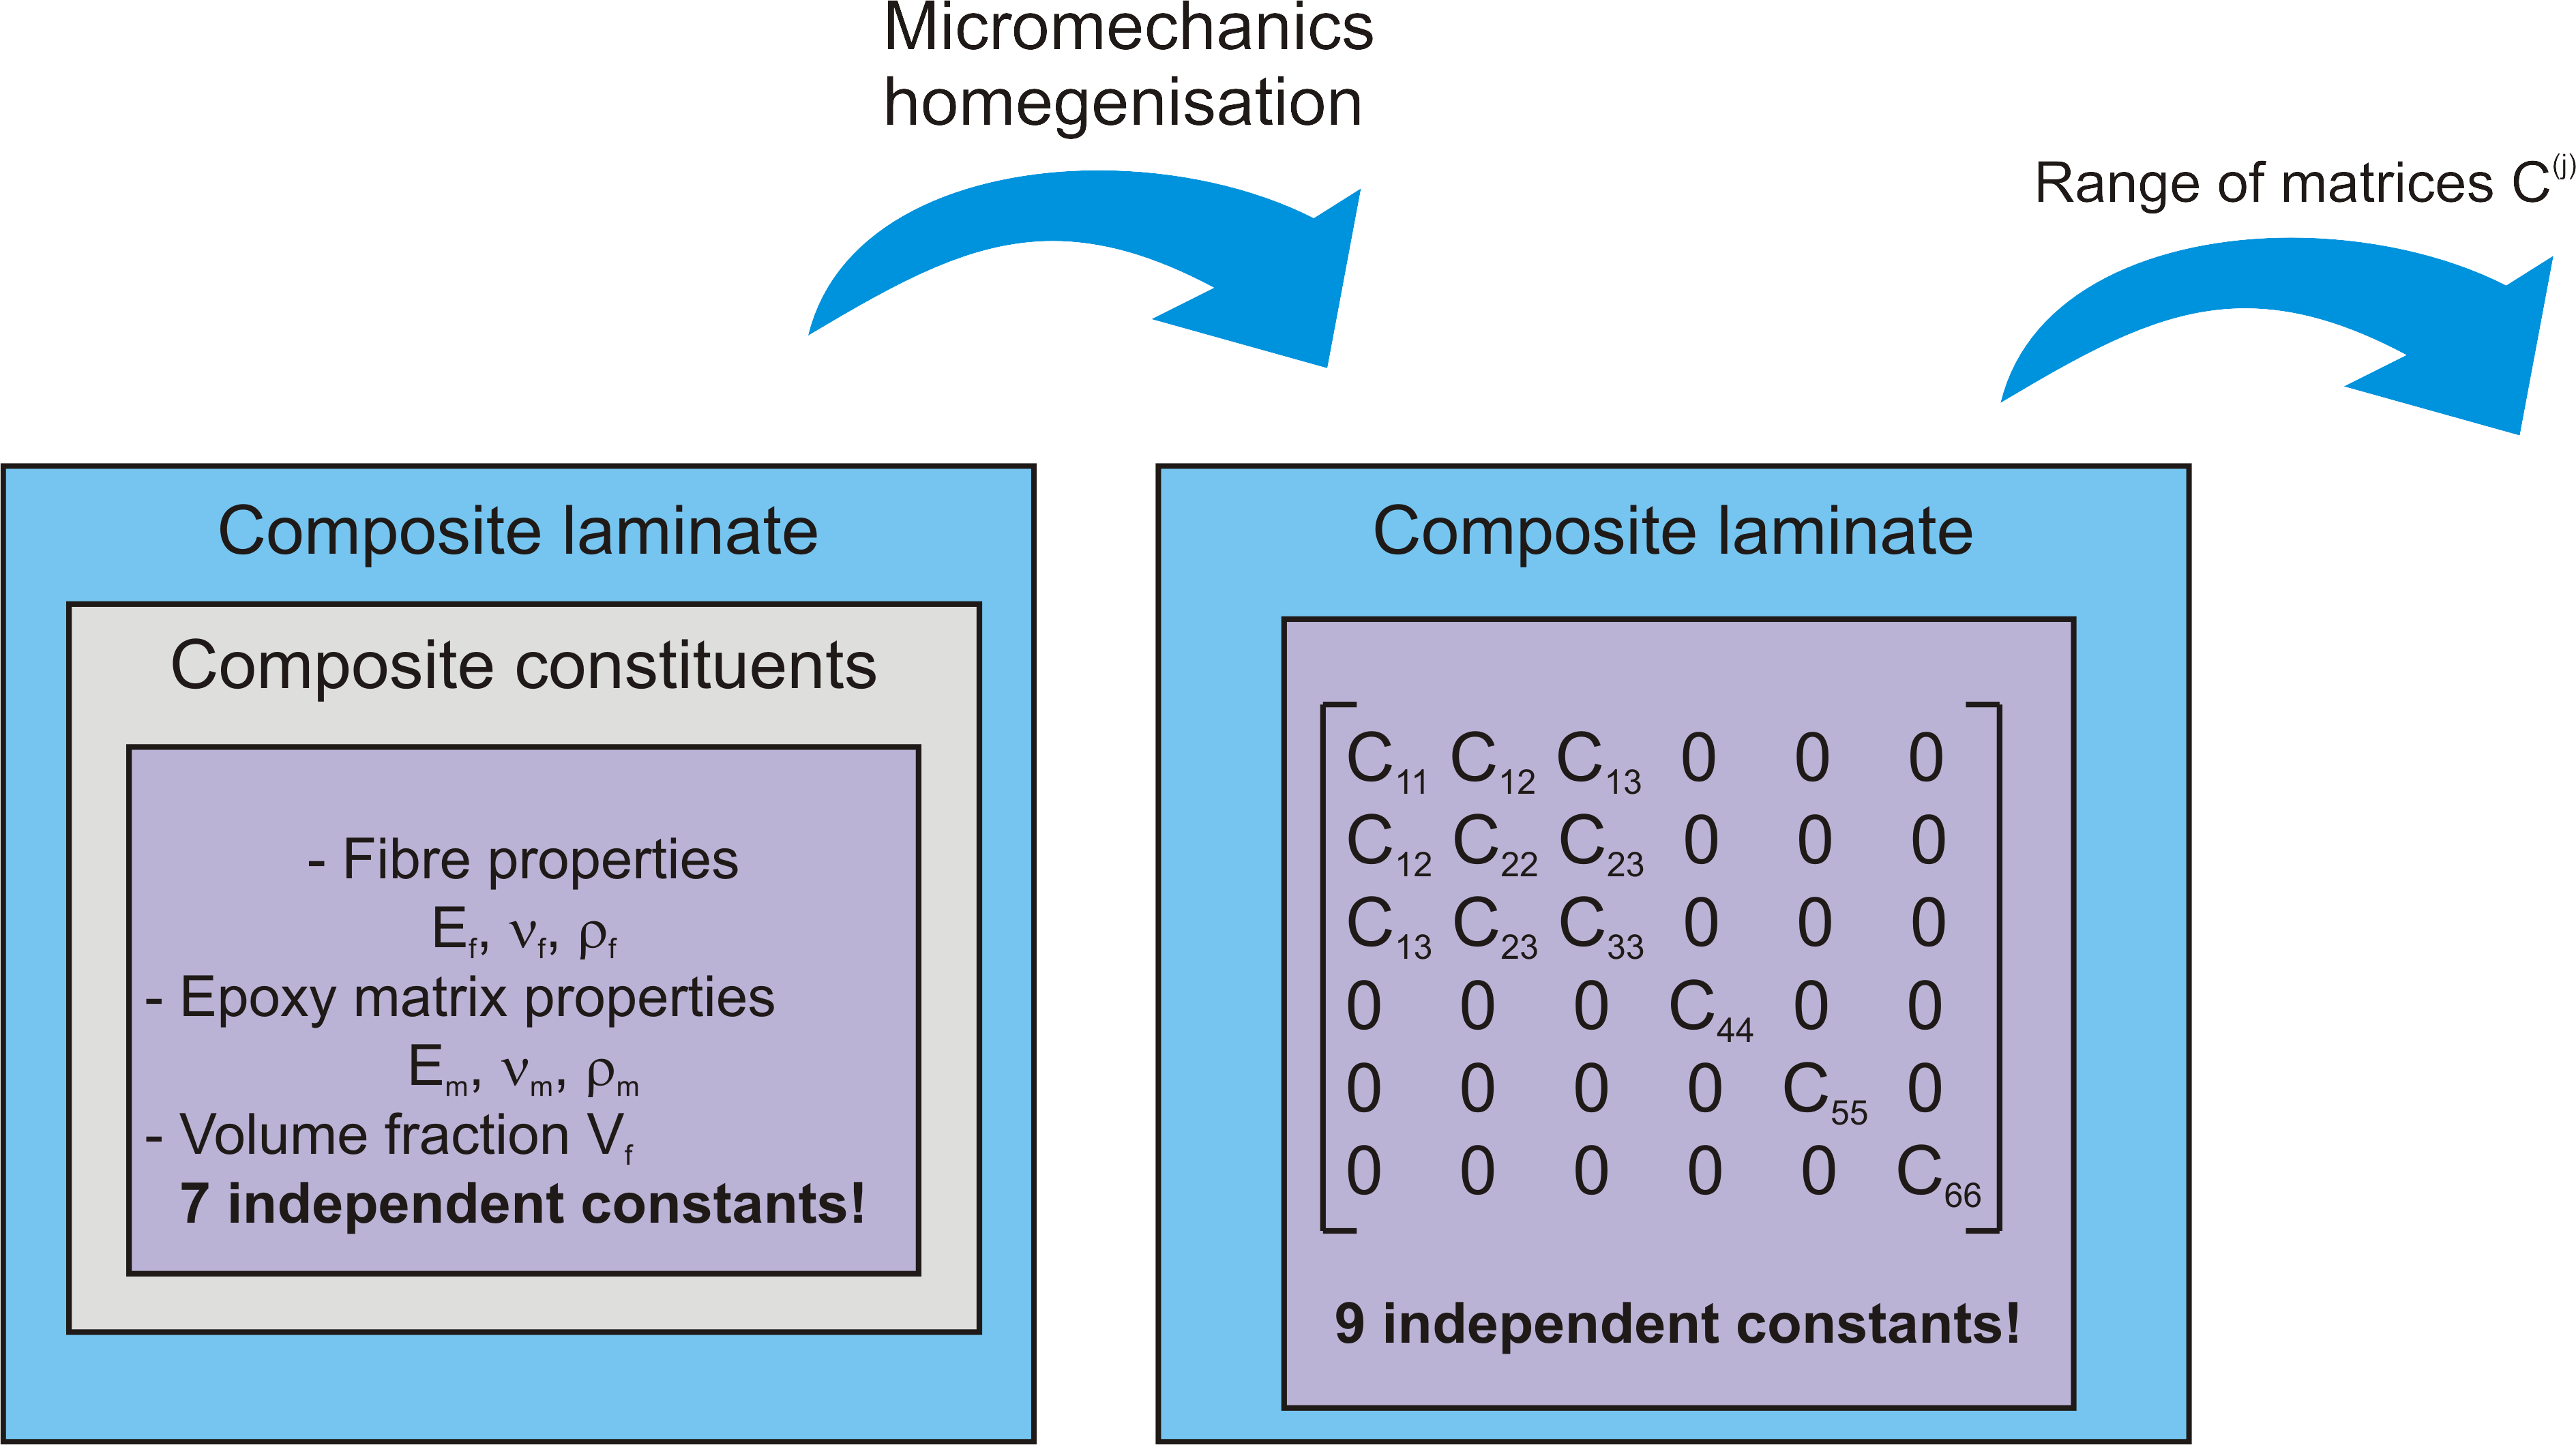
\includegraphics[width=\textwidth]{Plan-scheme4a.png}
	}
	\only<2>{
		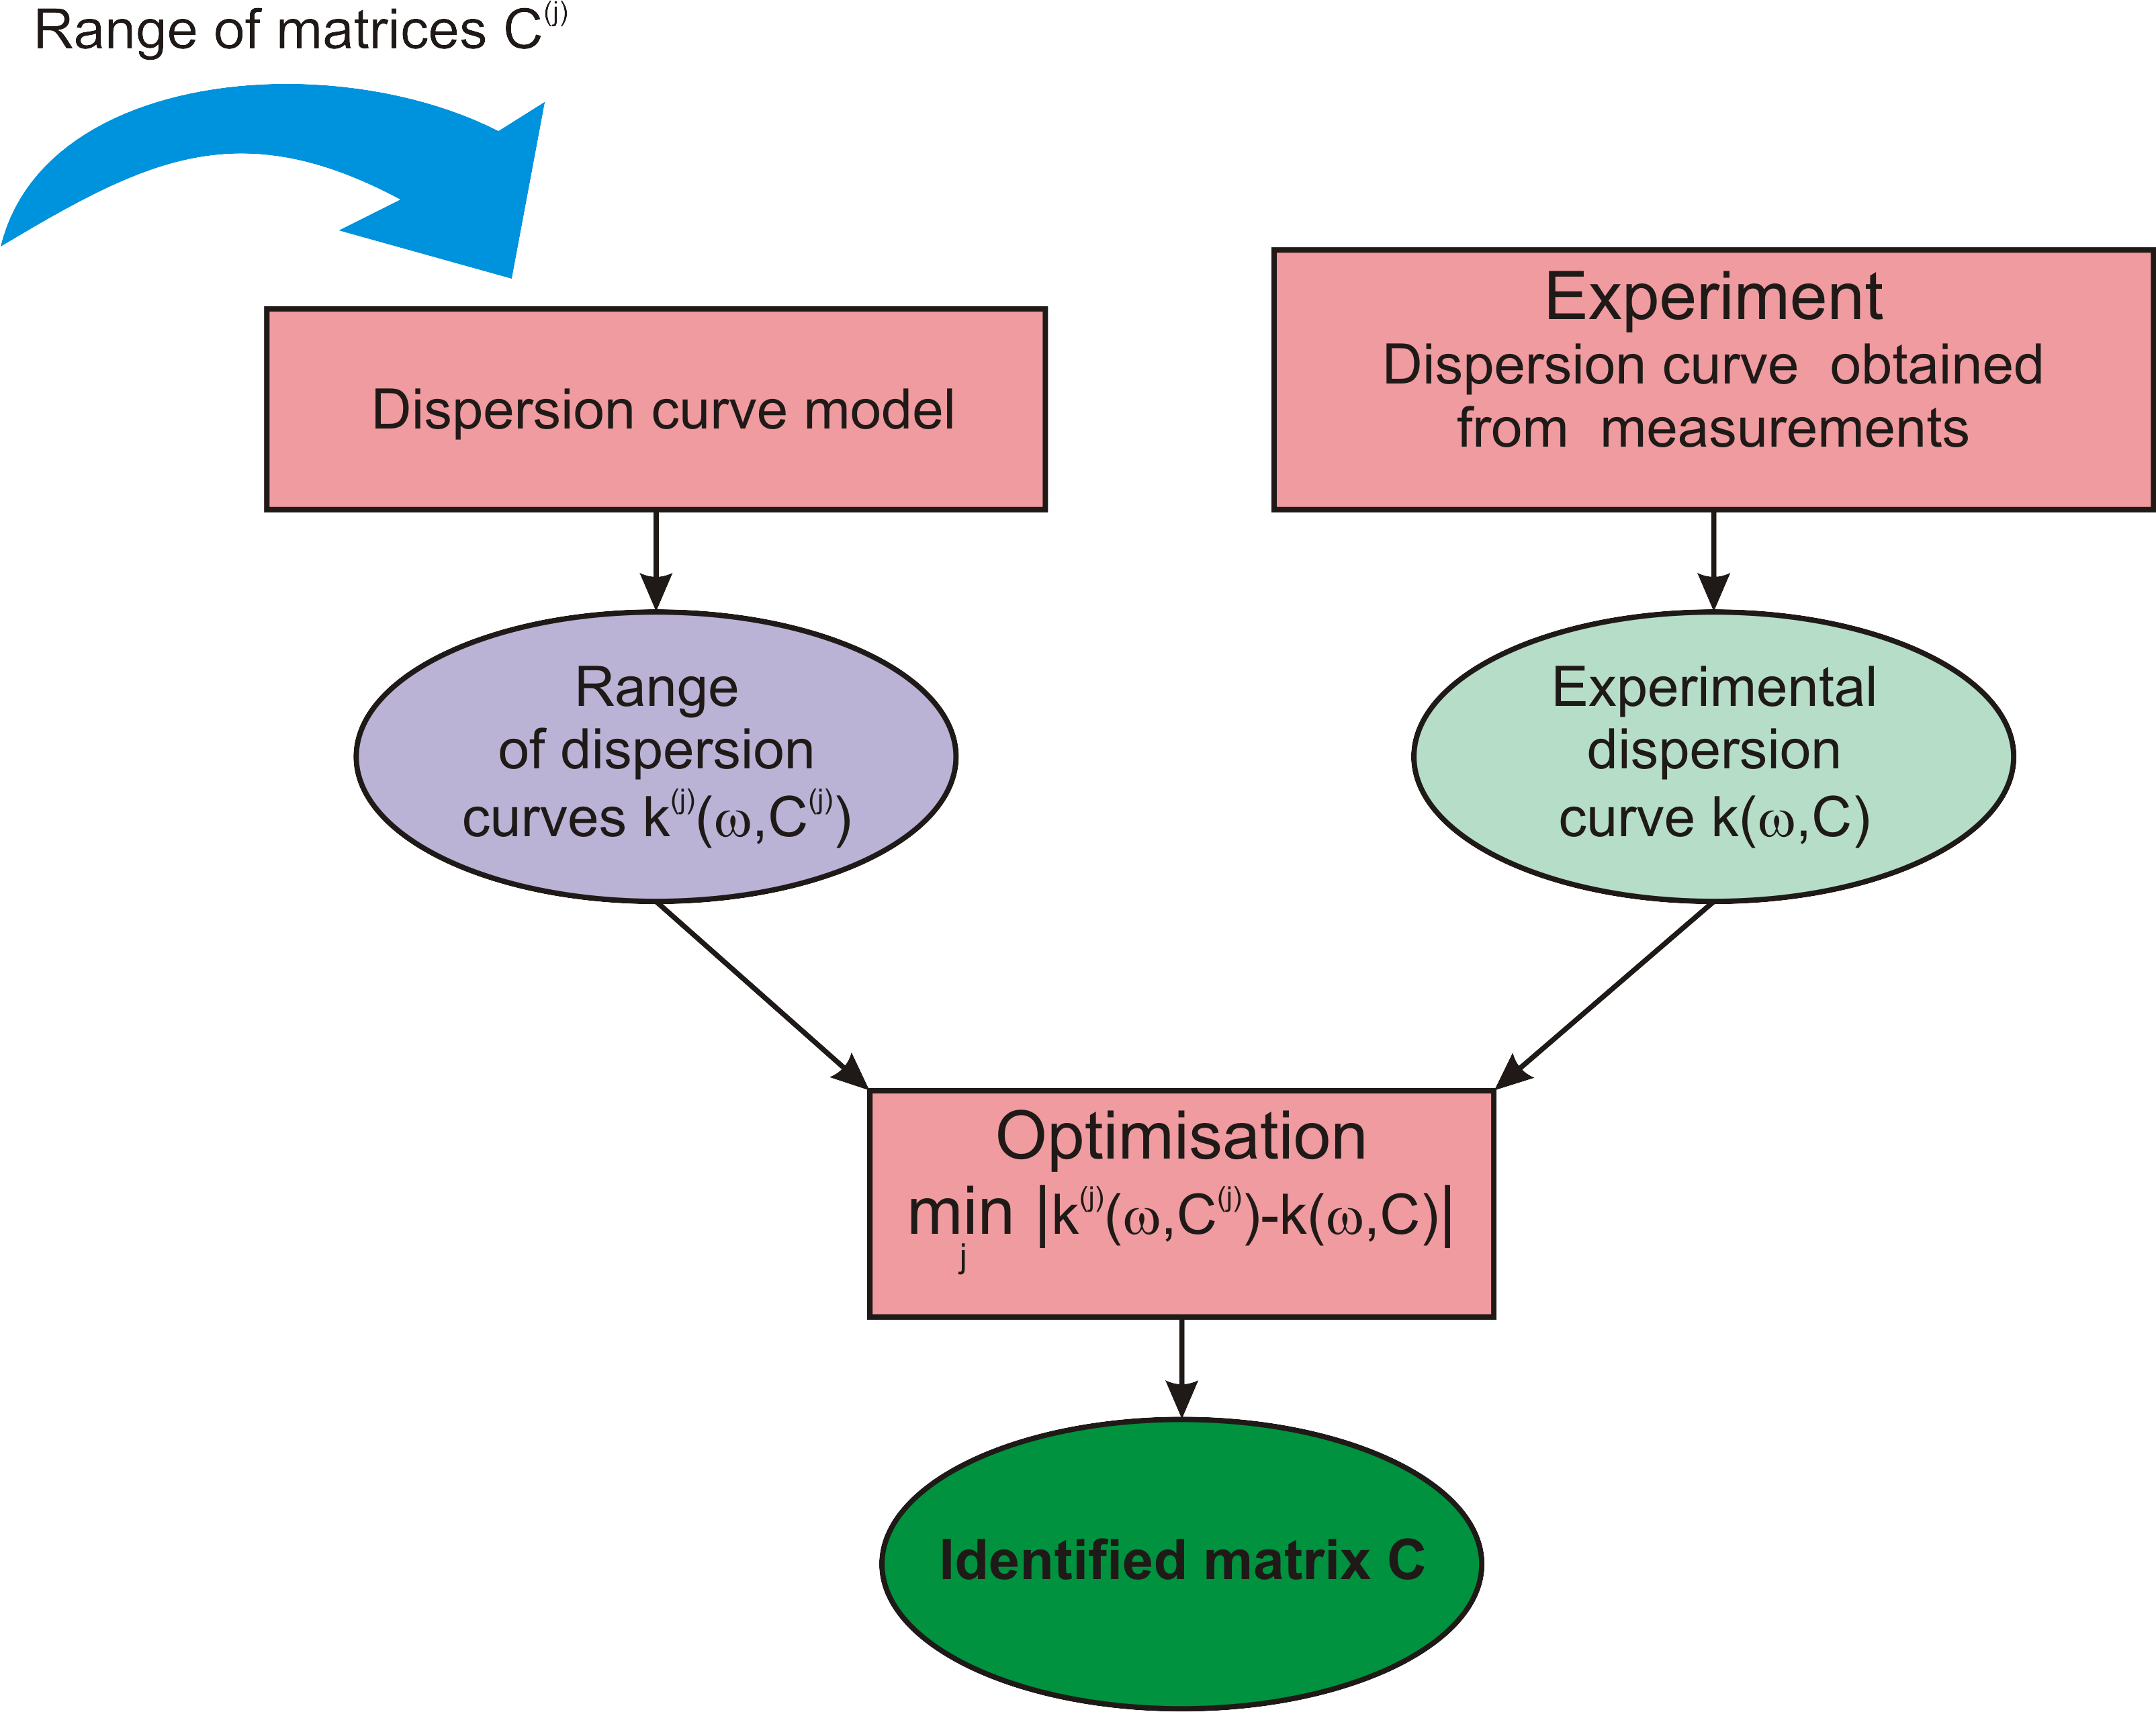
\includegraphics[width=0.9\textwidth]{Plan-scheme4b.png}
	}
\end{figure}
\only<1>{
	\begin{equation*}
	\bs{\sigma} = \matr{C} \, \bs{\varepsilon}
	\end{equation*}
}
\end{frame}
%%%%%%%%%%%%%%%%%%%%%%%%%%%%%%%%%%%%%%%%%%%%%%%%%%
%%%%%%%%%%%%%%%%%%%%%%%%%%%%%%%%%%%%%%%%%%%%%%%%%%
\begin{frame}[label=frame4]{Dispersion curves (1)}
	\begin{alertblock}{Definition}
		A \textbf{dispersion relation} relates the wavelength $\lambda$ or wavenumber $k$ of a wave to its frequency $\omega$.\\
		 \vspace{10pt}
		$k(\omega)$ $[\frac{1}{\mathrm{rad}}]$\\
			 \vspace{6pt}
		$k(f)$ $[\frac{1}{\mathrm{m}}]$
	\end{alertblock}
	\begin{block}{Phase velocity}
		\begin{equation*}
			c_p = \frac{\omega}{k}
		\end{equation*}
	\end{block}
\begin{block}{Group velocity}
	\begin{equation*}
	c_g = \frac{\drv \omega}{\drv k}
	\end{equation*}
\end{block}
\end{frame}
%%%%%%%%%%%%%%%%%%%%%%%%%%%%%%%%%%%%%%%%%%%%%%%%%%
\begin{frame}[label=frame5]{Dispersion curves (2)}
\newcommand{\modelname}{SASE2}
	\begin{figure}
		\only<1>{
		\includegraphics[width=\textwidth]{SASE/\modelname_out/\modelname_angle_30_exemplary_dispersion_curves.png}
		}
		\only<2>{
		\includegraphics[width=\textwidth]{SASE/\modelname_out/\modelname_angle_30_exemplary_dispersion_curves_sorted.png}
		}
	\end{figure}
\end{frame}
%%%%%%%%%%%%%%%%%%%%%%%%%%%%%%%%%%%%%%%%%%%%%%%%%%
\begin{frame}[label=frame6]{Dispersion curves (3)}
\def\myindenta{0.17\textwidth} % define myindenta variable  for correcting caption placement
\begin{columns}[T]
	\column{0.5\textwidth}
	\newcommand{\modelname}{dispersion_effect}
	\begin{figure}
		\includegraphics[width=0.9\textwidth]{SASE/\modelname_out/excitation_narrow_time.png}
		\includegraphics[width=0.9\textwidth]{SASE/\modelname_out/excitation_wide_time.png}
	\end{figure}
	\column{0.5\textwidth}
	\newcommand{\modelname}{dispersion_effect}
	\begin{figure}
			\includegraphics[width=0.9\textwidth]{SASE/\modelname_out/excitation_narrow_frequency.png}
			\includegraphics[width=0.9\textwidth]{SASE/\modelname_out/excitation_wide_frequency.png}
	\end{figure}
\end{columns}
\end{frame}
%%%%%%%%%%%%%%%%%%%%%%%%%%%%%%%%%%%%%%%%%%%%%%%%%%
\begin{frame}[label=frame7]{Dispersion curves (4)}
\def\myindenta{0.17\textwidth} % define myindenta variable  for correcting caption placement
\begin{columns}[T]
	\column{0.5\textwidth}
	\newcommand{\modelname}{dispersion_effect}
	\only<1>{
		\begin{figure}
			\includegraphics[width=\textwidth]{SASE/\modelname_out/A0_dispersion_less_dispersive.png}
			\caption{Less dispersive region}
		\end{figure}
		\column{0.5\textwidth}
		\newcommand{\modelname}{dispersion_effect}
		\begin{figure}
			\includegraphics[width=\textwidth]{SASE/\modelname_out/A0_dispersion_dispersive.png}
			\caption{Dispersive region}
		\end{figure}
	}
	\only<2>{
		\begin{figure}
			\includegraphics[width=\textwidth]{SASE/\modelname_out/A0_phase_velocity_less_dispersive.png}
			\caption{Less dispersive region}
		\end{figure}
		\column{0.5\textwidth}
		\newcommand{\modelname}{dispersion_effect}
		\begin{figure}
			\includegraphics[width=\textwidth]{SASE/\modelname_out/A0_phase_velocity_dispersive.png}
			\caption{Dispersive region}
		\end{figure}
	}
	\only<3>{
		\begin{figure}
			\includegraphics[width=\textwidth]{SASE/\modelname_out/A0_group_velocity_less_dispersive.png}
			\caption{Less dispersive region}
		\end{figure}
		\column{0.5\textwidth}
		\newcommand{\modelname}{dispersion_effect}
		\begin{figure}
			\includegraphics[width=\textwidth]{SASE/\modelname_out/A0_group_velocity_dispersive.png}
			\caption{Dispersive region}
		\end{figure}
	}
\end{columns}
\begin{center}
	\only<2>{\alert{Phase velocities}}
	\only<3>{\alert{Group velocities}}
\end{center}
\end{frame}
%%%%%%%%%%%%%%%%%%%%%%%%%%%%%%%%%%%%%%%%%%%%%%%%%%
\begin{frame}[label=frame8]{Dispersion curves (5)}
\def\myindenta{0.17\textwidth} % define myindenta variable  for correcting caption placement
	\newcommand{\modelname}{dispersion_effect}
	\only<1>{
	\begin{figure}
		\includegraphics[width=\textwidth]{SASE/\modelname_out/dispersion_effect_less_dispersive_L_1.png}
		\includegraphics[width=\textwidth]{SASE/\modelname_out/dispersion_effect_dispersive_L_1.png}
	\end{figure}
	}
	\only<2>{
		\begin{figure}
			\includegraphics[width=\textwidth]{SASE/\modelname_out/dispersion_effect_less_dispersive_L_2.png}
			\includegraphics[width=\textwidth]{SASE/\modelname_out/dispersion_effect_dispersive_L_2.png}
		\end{figure}
	}
	\only<3>{
		\begin{figure}
			\includegraphics[width=\textwidth]{SASE/\modelname_out/dispersion_effect_less_dispersive_L_3.png}
			\includegraphics[width=\textwidth]{SASE/\modelname_out/dispersion_effect_dispersive_L_3.png}
		\end{figure}
	}
	\only<4>{
		\begin{figure}
			\includegraphics[width=\textwidth]{SASE/\modelname_out/dispersion_effect_less_dispersive_L_4.png}
			\includegraphics[width=\textwidth]{SASE/\modelname_out/dispersion_effect_dispersive_L_4.png}
		\end{figure}
	}
	\only<5>{
		\begin{figure}
			\includegraphics[width=\textwidth]{SASE/\modelname_out/dispersion_effect_less_dispersive_L_5.png}
			\includegraphics[width=\textwidth]{SASE/\modelname_out/dispersion_effect_dispersive_L_5.png}
		\end{figure}
	}
	\only<6>{
		\begin{figure}
			\includegraphics[width=\textwidth]{SASE/\modelname_out/dispersion_effect_less_dispersive_L_6.png}
			\includegraphics[width=\textwidth]{SASE/\modelname_out/dispersion_effect_dispersive_L_6.png}
		\end{figure}
	}
	\only<7>{
	\begin{figure}
		\includegraphics[width=\textwidth]{SASE/\modelname_out/dispersion_effect_less_dispersive_L_7.png}
		\includegraphics[width=\textwidth]{SASE/\modelname_out/dispersion_effect_dispersive_L_7.png}
	\end{figure}
	}
	\only<8>{
		\begin{figure}
			\includegraphics[width=\textwidth]{SASE/\modelname_out/dispersion_effect_less_dispersive_L_8.png}
			\includegraphics[width=\textwidth]{SASE/\modelname_out/dispersion_effect_dispersive_L_8.png}
		\end{figure}
	}
	\only<9>{
		\begin{figure}
			\includegraphics[width=\textwidth]{SASE/\modelname_out/dispersion_effect_less_dispersive_L_9.png}
			\includegraphics[width=\textwidth]{SASE/\modelname_out/dispersion_effect_dispersive_L_9.png}
		\end{figure}
	}
	\only<10>{
		\begin{figure}
			\includegraphics[width=\textwidth]{SASE/\modelname_out/dispersion_effect_less_dispersive_L_10.png}
			\includegraphics[width=\textwidth]{SASE/\modelname_out/dispersion_effect_dispersive_L_10.png}
		\end{figure}
	}
	\only<11>{
		\begin{figure}
			\includegraphics[width=\textwidth]{SASE/\modelname_out/dispersion_effect_less_dispersive_L_11.png}
			\includegraphics[width=\textwidth]{SASE/\modelname_out/dispersion_effect_dispersive_L_11.png}
		\end{figure}
	}
\end{frame}
%%%%%%%%%%%%%%%%%%%%%%%%%%%%%%%%%%%%%%%%%%%%%%%%%%
\section{SASE for dispersion curves}
%%%%%%%%%%%%%%%%%%%%%%%%%%%%%%%%%%%%%%%%%%%%%%%%%%
\begin{frame}[label=frame9]{Semi Analytical Spectral Element Method (SASE)}
	\begin{figure}
		\includegraphics[width=\textwidth]{layered_composite_SASE.png}
	\end{figure}
	 \begin{equation*}
		\vect{u}(x,y,z,t) = \matr{U}(x) \exp \left[ i (\omega t + k \sin (\beta) y - k \cos (\beta) z)\right]
	\end{equation*}
\end{frame}
%%%%%%%%%%%%%%%%%%%%%%%%%%%%%%%%%%%%%%%%%%%%%%%%%%
\begin{frame}[t,label=frame10]{Semi Analytical Spectral Element Method (SASE)}
\only<1-3>{
	\begin{equation*}
		\left[\matr{A} - \omega^2\matr{M} \right] \vect{U} =0,
		\label{eq:eig_dispersion}
	\end{equation*}
where $\omega$ is the angular frequency, $\matr{M}$ is the mass matrix, $\matr{U}$ is the nodal displacement vector, and the matrix $\matr{A}$ can be defined as:
	\begin{equation*}
		\begin{aligned}
		\matr{A} & =  k^2\left(s^2 \,\matr{K}_{22} + c^2\, \matr{K}_{33} - c s\, \matr{K}_{23} - c s\, \matr{K}_{32}\right) \\
		& + i k\, \matr{T}^T\left(-c\, \matr{K}_{13} - s\, \matr{K}_{21} + s\, \matr{K}_{12} + c\, \matr{K}_{31}\right) \matr{T} +\matr{K}_{11},
		\end{aligned}
		\label{eq:dispersion}
	\end{equation*}
	where  $s = \sin(\beta)$, $c = \cos(\beta)$, $i = \sqrt{-1}$.
}
\only<2-3>{
	\begin{equation*}
		\matr{K}_{mn}^e= \int \limits_{(e)} \matr{B}_m^{T} \matr{C}^e \, \matr{B}_n\, \ud x
		\label{eq:stiffness_matrix_e}
	\end{equation*}
}
\only<3>{
	Possible solutions:
	\begin{columns}[T]
		\column{0.5\textwidth}
		\begin{itemize}
			\item standard eigenvalue problem $\omega (k)$
		\end{itemize}
		\column{0.5\textwidth}
		\begin{itemize}
		\item second-order polynomial eigenvalue problem $k(\omega)$
		\end{itemize}
	\end{columns}
}
\end{frame}
%%%%%%%%%%%%%%%%%%%%%%%%%%%%%%%%%%%%%%%%%%%%%%%%%%
\begin{frame}[t,label=frame11]{Semi Analytical Spectral Element Method (SASE)}
\only<1-2>{
	\begin{columns}[T]
		\column{0.5\textwidth}
		\begin{itemize}
			\item standard eigenvalue problem $\omega (k)$
			\item real $k$ -- real $\omega$
			\item only dispersion curves
		\end{itemize}
		\column{0.5\textwidth}
		\begin{itemize}
			\item second-order polynomial eigenvalue problem $k(\omega)$
			\item real $\omega$ -- complex $k$
			\item dispersion curves and attenuation (complex $\matr{C}$)
		\end{itemize}
	\end{columns}
\vspace{10pt}
	\begin{columns}[T]
		\column{0.5\textwidth}
			\begin{equation*}
				\left[\matr{A} - \omega^2\matr{M} \right]_{\alert{M}} \vect{U} =0
			\end{equation*}
		\column{0.5\textwidth}
			\begin{equation*}
				\left[\hat{\matr{A}} - k \hat{\matr{D}} \right]_{\alert{2M}} \hat{\vect{Q}} =0
			\end{equation*}
			\begin{equation*}
				\hat{\vect{Q}} =\left[\begin{array}{c} 
				\vect{U}\\
				k \vect{U}
				\end{array} \right]
			\end{equation*}
	\end{columns}
}
\only<2>{
\begin{flalign*}
		&\hat{\matr{A}} =\left[\begin{array}{cc} 
			0 & \matr{K}_{11} - \omega^2 \matr{M}\\
			\matr{K}_{11} - \omega^2 \matr{M} & -i \left( c	\, \matr{K}_{13} - s\, \matr{K}_{12}  + s\, \matr{K}_{21} - c \, \matr{K}_{31}   \right)
			\end{array} \right]   \\
		&\hat{\matr{D}} =\left[\begin{array}{cc} 
		\matr{K}_{11} - \omega^2 \matr{M} & 0\\
		0& - \left( s^2 \, \matr{K}_{22} + c^2 \,  \matr{K}_{33}  -s c \,  \matr{K}_{23}  -sc \, \matr{K}_{32}  \right)
		\end{array} \right]
\end{flalign*}
%\begin{equation*}
%\hat{\matr{A}} =\left[\begin{array}{cc} 
%0 & \matr{K}_{11} - \omega^2 \matr{M}\\
%\matr{K}_{11} - \omega^2 \matr{M} & -i \left( c	\, \matr{K}_{13} - s\, \matr{K}_{12}  + s\, \matr{K}_{21} - c \, \matr{K}_{31}   \right)
%\end{array} \right]   
%%\end{equation*}
%\begin{equation*}
%\hat{\matr{D}} =\left[\begin{array}{cc} 
%\matr{K}_{11} - \omega^2 \matr{M} & 0\\
%0& - \left( s^2 \, \matr{K}_{22} + c^2 \,  \matr{K}_{33}  -s c \,  \matr{K}_{23}  -sc \, \matr{K}_{32}  \right)
%\end{array} \right]
%\end{equation*}
}
\end{frame}
%%%%%%%%%%%%%%%%%%%%%%%%%%%%%%%%%%%%%%%%%%%%%%%%%%
\section{Experimental measurements}
%%%%%%%%%%%%%%%%%%%%%%%%%%%%%%%%%%%%%%%%%%%%%%%%%%
\begin{frame}[t,label=frame12]{Composite specimen}
\begin{columns}[T]
	\column{0.7\textwidth}
	{\small
			\begin{itemize}
			\item 16 layers set at the same angle \\
			\item carbon: Prepreg GG 205  P (fibres Toray FT 300 - 3K 200 tex) by G. Angeloni 
			\item epoxy resin: IMP503Z-HT by Impregnatex Compositi 
			\item dimensions: 1200$\times$1200$\times$3.9 mm\\
			\item total weight:  8550 g
			\item density: 1522.4~kg/m\textsuperscript{3}
		\end{itemize}
	}
	\column{0.3\textwidth}
	\begin{figure}
		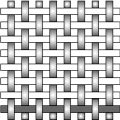
\includegraphics[width=0.9\textwidth]{weave-1.jpg}
		\caption{Plain weave fabric}
	\end{figure}
	\end{columns}
\begin{table}[h]
	\renewcommand{\arraystretch}{1.1}
	\centering \footnotesize
	\caption{Geometry of a plain weave fabric reinforced composite [mm]}
	%\begin{tabular}{@{}ccccccc@{}} % remove spaces from vertical lines
	\begin{tabular}{cccccc} 
		%\hline
		\toprule
		\multicolumn{4}{c}{\textbf{width} }	& \multicolumn{2}{c}{\textbf{thickness} }  \\ 
		%	\hline \hline
		\cmidrule(lr){1-4} \cmidrule(lr){5-6} 
		fill & warp & fill gap& warp gap& fill & warp\\
		%\hline
		$a_f$ &$a_w$& $g_f$  & $g_w$  & $h_f$& $h_w$ \\ 
		%\hline
		%\midrule
		\cmidrule(lr){1-2} \cmidrule(lr){3-4} \cmidrule(lr){5-6}
		1.92 &2.0& 0.05& 0.05 & 0.121875 & 0.121875 \\
		%\hline 
		\bottomrule 
	\end{tabular} 
	\label{tab:weave_geo}
\end{table}
\end{frame}
%%%%%%%%%%%%%%%%%%%%%%%%%%%%%%%%%%%%%%%%%%%%%%%%%%
\begin{frame}[t,label=frame13]{SLDV measurements and processing}
	\begin{figure}
	\makebox[\textwidth][c]{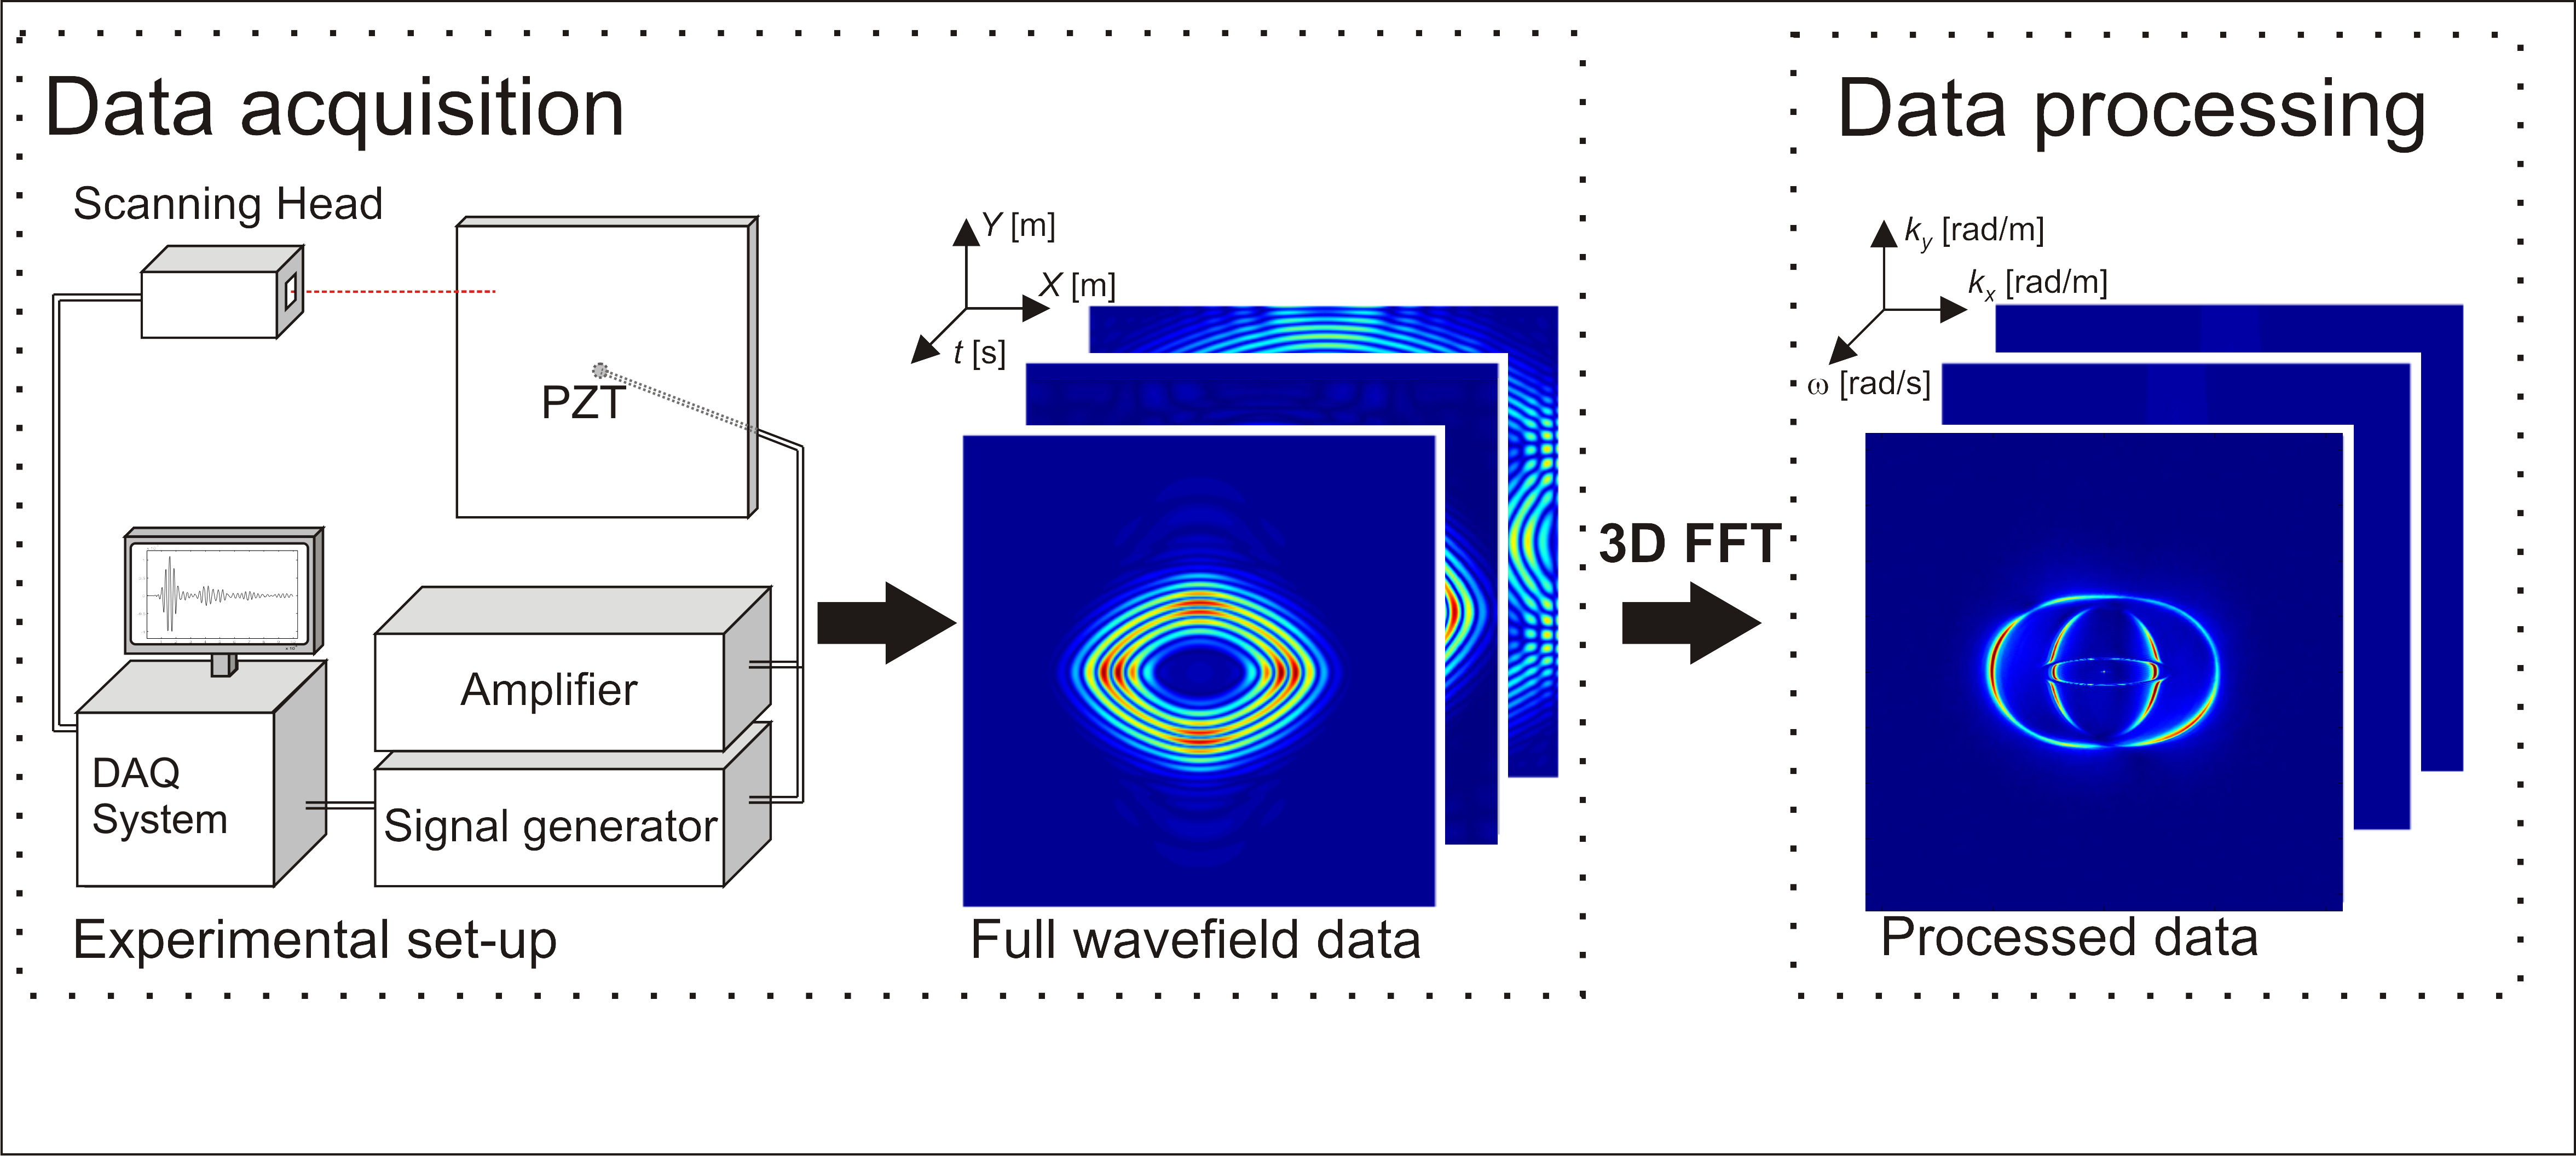
\includegraphics[width=1.15\textwidth]{Full_wavefield_2_dispersion_curves_experiment.png}}
	\end{figure}
\end{frame}
%%%%%%%%%%%%%%%%%%%%%%%%%%%%%%%%%%%%%%%%%%%%%%%%%%
\begin{frame}[t,label=frame14]{SLDV measurements}
\begin{columns}[T]
	\column{0.5\textwidth}
	\begin{figure}
	\includegraphics[width=\textwidth]{wibrometr-laserowy-1d_small-description.png}
	\end{figure}
	\column{0.5\textwidth}
	\begin{enumerate}
	\item Signal generator: TTI 1241 
	\item Amplifier: Piezo Systems EPA-104-230 $\pm$200 Vp
	\item Specimen
	\item Scanning head: Polytec PSV-400
	\item DAQ system: Polytec
	\end{enumerate}
\end{columns}
{\small
 Vibrometer allows measurements of vibration velocities in range 0.01~$\mu$m/s $-$ 10 m/s for frequencies from DC up to 1.5~MHz for measuring distance from 40~cm up to dozens of meters. Scanning resolution is 0.002$^{\circ}$  which provides possibility of defining about 300 000 points in laser working area.}\end{frame}
%%%%%%%%%%%%%%%%%%%%%%%%%%%%%%%%%%%%%%%%%%%%%%%%%%
\begin{frame}[t,label=frame15]{Experimental dispersion curves}
\begin{figure} [h!]
	\newcommand{\modelname}{ga_plain_weave_known_mass}
	\centering
		\includegraphics[width=0.9\textwidth]{genetic_algorithm/\modelname_out/\modelname_angle_60_dispersion_curves_initial_large.png}
		\caption{Numerical dispersion curves calculated for initial parameters overlayed on experimental data}
		\label{fig:dispersion60deg_initial}
\end{figure}
\end{frame}
%%%%%%%%%%%%%%%%%%%%%%%%%%%%%%%%%%%%%%%%%%%%%%%%%%
\section{Parametric studies}
%%%%%%%%%%%%%%%%%%%%%%%%%%%%%%%%%%%%%%%%%%%%%%%%%%
%%%%%%%%%%%%%%%%%%%%%%%%%%%%%%%%%%%%%%%%%%%%%%%%%%
\begin{frame}[t,label=frame16]{Variability of parameters}
\begin{table}
	\label{tab:mat_prop}
	\renewcommand{\arraystretch}{1.1}
	\centering \footnotesize
	\caption{Initial material properties of composite laminate}
	\begin{tabular}{ccccccc} 
		\toprule
		\multicolumn{3}{c}{\textbf{Matrix} }	& \multicolumn{3}{c}{\textbf{Fibres} } & \textbf{Volume fraction}	 \\ 
		\midrule
		$\rho_m$ & $E_m$ & $\nu_m$  & $\rho_f$ & $E_f$ & $\nu_f$ & $V$\\
		kg/m\textsuperscript{3} &GPa& --  & kg/m\textsuperscript{3}  & GPa& -- & \%\\ 
		\cmidrule(lr){1-3} \cmidrule(lr){4-6} \cmidrule(lr){7-7}
		1250 &3.43& 0.35& 1900 & 240 & 0.2 & 50\\
		\bottomrule 
	\end{tabular} 
\end{table}
\vspace{10pt}
\centering
\Large $\pm$20\%\\ 
\vspace{10pt}
\normalsize Influence on dispersion curves
\end{frame}
%%%%%%%%%%%%%%%%%%%%%%%%%%%%%%%%%%%%%%%%%%%%%%%%%%
\begin{frame}[t,label=frame17]{SASE dispersion curves: density influence}
%\vspace{6pt}
\def\myindenta{0.17\textwidth} % define myindenta variable  for correcting caption placement
\begin{columns}[T]
	\column{0.5\textwidth}
	\newcommand{\modelname}{SASE2}
		\begin{figure}
			\only<1>{
			\includegraphics[width=\textwidth]{SASE/\modelname_out/\modelname_angle_0_param_dispersion_curves.png}
			\caption{\hspace{\myindenta}The influence of \alert{matrix density}\\ \hspace{\myindenta}on dispersion curves at angle \textbf{0}$^{\circ}$}
			}
			\only<2>{
			\includegraphics[width=\textwidth]{SASE/\modelname_out/\modelname_angle_15_param_dispersion_curves.png}
			\caption{\hspace{\myindenta}The influence of \alert{matrix density}\\ \hspace{\myindenta}on dispersion curves at angle \textbf{15}$^{\circ}$ }
			}
			\only<3>{
			\includegraphics[width=\textwidth]{SASE/\modelname_out/\modelname_angle_30_param_dispersion_curves.png}
			\caption{\hspace{\myindenta}The influence of \alert{matrix density}\\ \hspace{\myindenta}on dispersion curves at angle \textbf{30}$^{\circ}$ }
			}
		    \only<4>{
		    	\includegraphics[width=\textwidth]{SASE/\modelname_out/\modelname_angle_45_param_dispersion_curves.png}
		    	\caption{\hspace{\myindenta}The influence of \alert{matrix density}\\ \hspace{\myindenta}on dispersion curves at angle \textbf{45}$^{\circ}$ }
		    }
	    	\only<5>{
	    		\includegraphics[width=\textwidth]{SASE/\modelname_out/\modelname_angle_60_param_dispersion_curves.png}
	    		\caption{\hspace{\myindenta}The influence of \alert{matrix density}\\ \hspace{\myindenta}on dispersion curves at angle \textbf{60}$^{\circ}$ }
	    	}
    		\only<6>{
    			\includegraphics[width=\textwidth]{SASE/\modelname_out/\modelname_angle_75_param_dispersion_curves.png}
    			\caption{\hspace{\myindenta}The influence of \alert{matrix density}\\ \hspace{\myindenta}on dispersion curves at angle \textbf{75}$^{\circ}$ }
    		}
    		\only<7->{
    			\includegraphics[width=\textwidth]{SASE/\modelname_out/\modelname_angle_90_param_dispersion_curves.png}
    			\caption{\hspace{\myindenta}The influence of \alert{matrix density}\\ \hspace{\myindenta}on dispersion curves at angle \textbf{90}$^{\circ}$ }
    		}
			\label{fig:rhom}
		\end{figure}
	\column{0.5\textwidth}
	\newcommand{\modelname}{SASE3}
		\begin{figure}
			\only<1>{
			\includegraphics[width=\textwidth]{SASE/\modelname_out/\modelname_angle_0_param_dispersion_curves.png}
			\caption{\hspace{\myindenta}The influence of \alert{fibre density}\\ \hspace{\myindenta}on dispersion curves at angle \textbf{0}$^{\circ}$}
			}
			\only<2>{
			\includegraphics[width=\textwidth]{SASE/\modelname_out/\modelname_angle_15_param_dispersion_curves.png}
			\caption{\hspace{\myindenta}The influence of \alert{fibre density}\\ \hspace{\myindenta}on dispersion curves at angle \textbf{15}$^{\circ}$}
			}
			\only<3>{
				\includegraphics[width=\textwidth]{SASE/\modelname_out/\modelname_angle_30_param_dispersion_curves.png}
				\caption{\hspace{\myindenta}The influence of \alert{fibre density}\\ \hspace{\myindenta}on dispersion curves at angle \textbf{30}$^{\circ}$}
			}
			\only<4>{
				\includegraphics[width=\textwidth]{SASE/\modelname_out/\modelname_angle_45_param_dispersion_curves.png}
				\caption{\hspace{\myindenta}The influence of \alert{fibre density}\\ \hspace{\myindenta}on dispersion curves at angle \textbf{45}$^{\circ}$}
			}
			\only<5>{
				\includegraphics[width=\textwidth]{SASE/\modelname_out/\modelname_angle_60_param_dispersion_curves.png}
				\caption{\hspace{\myindenta}The influence of \alert{fibre density}\\ \hspace{\myindenta}on dispersion curves at angle \textbf{60}$^{\circ}$}
			}
			\only<6>{
				\includegraphics[width=\textwidth]{SASE/\modelname_out/\modelname_angle_75_param_dispersion_curves.png}
				\caption{\hspace{\myindenta}The influence of \alert{fibre density}\\ \hspace{\myindenta}on dispersion curves at angle \textbf{75}$^{\circ}$}
			}
			\only<7->{
				\includegraphics[width=\textwidth]{SASE/\modelname_out/\modelname_angle_90_param_dispersion_curves.png}
				\caption{\hspace{\myindenta}The influence of \alert{fibre density}\\ \hspace{\myindenta}on dispersion curves at angle \textbf{90}$^{\circ}$}
			}
			\label{fig:rhof}
		\end{figure}
\end{columns}
	\only<8>{
	\begin{alertblock}{Remarks}
		\textbf{Fibres density} has slightly more influence on dispersion curves than \textbf{matrix density}.
	\end{alertblock}
	}
\end{frame}
%%%%%%%%%%%%%%%%%%%%%%%%%%%%%%%%%%%%%%%%%%%%%%%%%%
\begin{frame}[t,label=frame18]{SASE dispersion curves: Young modulus influence}
%\vspace{6pt}
\def\myindenta{0.12\textwidth} % define myindenta variable  for correcting caption placement

\begin{columns}[T]
	\column{0.5\textwidth}
	\newcommand{\modelname}{SASE4}
	\begin{figure}
		\only<1>{
			\includegraphics[width=\textwidth]{SASE/\modelname_out/\modelname_angle_0_param_dispersion_curves.png}
			\caption{\hspace{\myindenta}The influence of \alert{Young's modulus}\\ \hspace{\myindenta}\alert{of matrix} on dispersion curves at\\ \hspace{\myindenta}angle \textbf{0}$^{\circ}$}
		}
		\only<2>{
			\includegraphics[width=\textwidth]{SASE/\modelname_out/\modelname_angle_15_param_dispersion_curves.png}
			\caption{\hspace{\myindenta}The influence of \alert{Young's modulus}\\ \hspace{\myindenta}\alert{of matrix} on dispersion curves at\\ \hspace{\myindenta}angle \textbf{15}$^{\circ}$ }
		}
		\only<3>{
			\includegraphics[width=\textwidth]{SASE/\modelname_out/\modelname_angle_30_param_dispersion_curves.png}
			\caption{\hspace{\myindenta}The influence of \alert{Young's modulus}\\ \hspace{\myindenta}\alert{of matrix} on dispersion curves at\\ \hspace{\myindenta}angle \textbf{30}$^{\circ}$ }
		}
		\only<4>{
			\includegraphics[width=\textwidth]{SASE/\modelname_out/\modelname_angle_45_param_dispersion_curves.png}
			\caption{\hspace{\myindenta}The influence of \alert{Young's modulus}\\ \hspace{\myindenta}\alert{of matrix} on dispersion curves at\\ \hspace{\myindenta}angle \textbf{45}$^{\circ}$ }
		}
		\only<5>{
			\includegraphics[width=\textwidth]{SASE/\modelname_out/\modelname_angle_60_param_dispersion_curves.png}
			\caption{\hspace{\myindenta}The influence of \alert{Young's modulus}\\ \hspace{\myindenta}\alert{of matrix} on dispersion curves at\\ \hspace{\myindenta}angle \textbf{60}$^{\circ}$ }
		}
		\only<6>{
			\includegraphics[width=\textwidth]{SASE/\modelname_out/\modelname_angle_75_param_dispersion_curves.png}
			\caption{\hspace{\myindenta}The influence of \alert{Young's modulus}\\ \hspace{\myindenta}\alert{of matrix} on dispersion curves at\\ \hspace{\myindenta}angle \textbf{75}$^{\circ}$ }
		}
		\only<7->{
			\includegraphics[width=\textwidth]{SASE/\modelname_out/\modelname_angle_90_param_dispersion_curves.png}
			\caption{\hspace{\myindenta}The influence of \alert{Young's modulus}\\ \hspace{\myindenta}\alert{of matrix} on dispersion curves at\\ \hspace{\myindenta}angle \textbf{90}$^{\circ}$ }
		}
		\label{fig:em}
	\end{figure}
	\column{0.5\textwidth}
	\newcommand{\modelname}{SASE5}
	\begin{figure}
		\only<1>{
			\includegraphics[width=\textwidth]{SASE/\modelname_out/\modelname_angle_0_param_dispersion_curves.png}
			\caption{\hspace{\myindenta}The influence of \alert{Young's modulus}\\ \hspace{\myindenta}\alert{of fibres} on dispersion curves at\\ \hspace{\myindenta}angle \textbf{0}$^{\circ}$}
		}
		\only<2>{
			\includegraphics[width=\textwidth]{SASE/\modelname_out/\modelname_angle_15_param_dispersion_curves.png}
			\caption{\hspace{\myindenta}The influence of \alert{Young's modulus}\\ \hspace{\myindenta}\alert{of fibres} on dispersion curves at\\ \hspace{\myindenta}angle \textbf{15}$^{\circ}$}
		}
		\only<3>{
			\includegraphics[width=\textwidth]{SASE/\modelname_out/\modelname_angle_30_param_dispersion_curves.png}
			\caption{\hspace{\myindenta}The influence of \alert{Young's modulus}\\ \hspace{\myindenta}\alert{of fibres} on dispersion curves at\\ \hspace{\myindenta}angle \textbf{30}$^{\circ}$}
		}
		\only<4>{
			\includegraphics[width=\textwidth]{SASE/\modelname_out/\modelname_angle_45_param_dispersion_curves.png}
			\caption{\hspace{\myindenta}The influence of \alert{Young's modulus}\\ \hspace{\myindenta}\alert{of fibres} on dispersion curves at\\ \hspace{\myindenta}angle \textbf{45}$^{\circ}$}
		}
		\only<5>{
			\includegraphics[width=\textwidth]{SASE/\modelname_out/\modelname_angle_60_param_dispersion_curves.png}
			\caption{\hspace{\myindenta}The influence of \alert{Young's modulus}\\ \hspace{\myindenta}\alert{of fibres} on dispersion curves at\\ \hspace{\myindenta}angle \textbf{60}$^{\circ}$}
		}
		\only<6>{
			\includegraphics[width=\textwidth]{SASE/\modelname_out/\modelname_angle_75_param_dispersion_curves.png}
			\caption{\hspace{\myindenta}The influence of \alert{Young's modulus}\\ \hspace{\myindenta}\alert{of fibres} on dispersion curves at\\ \hspace{\myindenta}angle \textbf{75}$^{\circ}$}
		}
		\only<7->{
			\includegraphics[width=\textwidth]{SASE/\modelname_out/\modelname_angle_90_param_dispersion_curves.png}
			\caption{\hspace{\myindenta}The influence of \alert{Young's modulus}\\ \hspace{\myindenta}\alert{of fibres} on dispersion curves at\\ \hspace{\myindenta}angle \textbf{90}$^{\circ}$}
		}
		\label{fig:ef}
	\end{figure}
\end{columns}
\only<8>{
	\begin{alertblock}{Remarks}
		\textbf{Young's modulus of matrix} has much more influence on dispersion curves than \textbf{Young's modulus of fibres}.
	\end{alertblock}
}
\end{frame}
%%%%%%%%%%%%%%%%%%%%%%%%%%%%%%%%%%%%%%%%%%%%%%%%%%
\begin{frame}[t,label=frame19]{SASE dispersion curves: Poisson's ratio influence}
%\vspace{6pt}
\def\myindenta{0.12\textwidth} % define myindenta variable  for correcting caption placement
\begin{columns}[T]
	\column{0.5\textwidth}
	\newcommand{\modelname}{SASE6}
	\begin{figure}
		\only<1>{
			\includegraphics[width=\textwidth]{SASE/\modelname_out/\modelname_angle_0_param_dispersion_curves.png}
			\caption{\hspace{\myindenta}The influence of \alert{Poisson's ratio}\\ \hspace{\myindenta}\alert{of matrix} on dispersion curves at\\ \hspace{\myindenta}angle \textbf{0}$^{\circ}$}
		}
		\only<2>{
			\includegraphics[width=\textwidth]{SASE/\modelname_out/\modelname_angle_15_param_dispersion_curves.png}
			\caption{\hspace{\myindenta}The influence of \alert{Poisson's ratio}\\ \hspace{\myindenta}\alert{of matrix} on dispersion curves at\\ \hspace{\myindenta}angle \textbf{15}$^{\circ}$ }
		}
		\only<3>{
			\includegraphics[width=\textwidth]{SASE/\modelname_out/\modelname_angle_30_param_dispersion_curves.png}
			\caption{\hspace{\myindenta}The influence of \alert{Poisson's ratio}\\ \hspace{\myindenta}\alert{of matrix} on dispersion curves at\\ \hspace{\myindenta}angle \textbf{30}$^{\circ}$ }
		}
		\only<4>{
			\includegraphics[width=\textwidth]{SASE/\modelname_out/\modelname_angle_45_param_dispersion_curves.png}
			\caption{\hspace{\myindenta}The influence of \alert{Poisson's ratio}\\ \hspace{\myindenta}\alert{of matrix} on dispersion curves at\\ \hspace{\myindenta}angle \textbf{45}$^{\circ}$ }
		}
		\only<5>{
			\includegraphics[width=\textwidth]{SASE/\modelname_out/\modelname_angle_60_param_dispersion_curves.png}
			\caption{\hspace{\myindenta}The influence of \alert{Poisson's ratio}\\ \hspace{\myindenta}\alert{of matrix} on dispersion curves at\\ \hspace{\myindenta}angle \textbf{60}$^{\circ}$ }
		}
		\only<6>{
			\includegraphics[width=\textwidth]{SASE/\modelname_out/\modelname_angle_75_param_dispersion_curves.png}
			\caption{\hspace{\myindenta}The influence of \alert{Poisson's ratio}\\ \hspace{\myindenta}\alert{of matrix} on dispersion curves at\\ \hspace{\myindenta}angle \textbf{75}$^{\circ}$ }
		}
		\only<7->{
			\includegraphics[width=\textwidth]{SASE/\modelname_out/\modelname_angle_90_param_dispersion_curves.png}
			\caption{\hspace{\myindenta}The influence of \alert{Poisson's ratio}\\ \hspace{\myindenta}\alert{of matrix} on dispersion curves at\\ \hspace{\myindenta}angle \textbf{90}$^{\circ}$ }
		}
		\label{fig:nim}
	\end{figure}
	\column{0.5\textwidth}
	\newcommand{\modelname}{SASE7}
	\begin{figure}
		\only<1>{
			\includegraphics[width=\textwidth]{SASE/\modelname_out/\modelname_angle_0_param_dispersion_curves.png}
			\caption{\hspace{\myindenta}The influence of \alert{Poisson's ratio}\\ \hspace{\myindenta}\alert{of fibres} on dispersion curves at\\ \hspace{\myindenta}angle \textbf{0}$^{\circ}$}
		}
		\only<2>{
			\includegraphics[width=\textwidth]{SASE/\modelname_out/\modelname_angle_15_param_dispersion_curves.png}
			\caption{\hspace{\myindenta}The influence of \alert{Poisson's ratio}\\ \hspace{\myindenta}\alert{of fibres} on dispersion curves at\\ \hspace{\myindenta}angle \textbf{15}$^{\circ}$}
		}
		\only<3>{
			\includegraphics[width=\textwidth]{SASE/\modelname_out/\modelname_angle_30_param_dispersion_curves.png}
			\caption{\hspace{\myindenta}The influence of \alert{Poisson's ratio}\\ \hspace{\myindenta}\alert{of fibres} on dispersion curves at\\ \hspace{\myindenta}angle \textbf{30}$^{\circ}$}
		}
		\only<4>{
			\includegraphics[width=\textwidth]{SASE/\modelname_out/\modelname_angle_45_param_dispersion_curves.png}
			\caption{\hspace{\myindenta}The influence of \alert{Poisson's ratio}\\ \hspace{\myindenta}\alert{of fibres} on dispersion curves at\\ \hspace{\myindenta}angle \textbf{45}$^{\circ}$}
		}
		\only<5>{
			\includegraphics[width=\textwidth]{SASE/\modelname_out/\modelname_angle_60_param_dispersion_curves.png}
			\caption{\hspace{\myindenta}The influence of \alert{Poisson's ratio}\\ \hspace{\myindenta}\alert{of fibres} on dispersion curves at\\ \hspace{\myindenta}angle \textbf{60}$^{\circ}$}
		}
		\only<6>{
			\includegraphics[width=\textwidth]{SASE/\modelname_out/\modelname_angle_75_param_dispersion_curves.png}
			\caption{\hspace{\myindenta}The influence of \alert{Poisson's ratio}\\ \hspace{\myindenta}\alert{of fibres} on dispersion curves at\\ \hspace{\myindenta}angle \textbf{75}$^{\circ}$}
		}
		\only<7->{
			\includegraphics[width=\textwidth]{SASE/\modelname_out/\modelname_angle_90_param_dispersion_curves.png}
			\caption{\hspace{\myindenta}The influence of \alert{Poisson's ratio}\\ \hspace{\myindenta}\alert{of fibres} on dispersion curves at\\ \hspace{\myindenta}angle \textbf{90}$^{\circ}$}
		}
		\label{fig:nif}
	\end{figure}
\end{columns}
\only<8>{
	\begin{alertblock}{Remarks}
		\textbf{Poisson's ratio of fibres} is the least influential parameter on dispersion curves among investigated parameters.
	\end{alertblock}
}
\end{frame}
%%%%%%%%%%%%%%%%%%%%%%%%%%%%%%%%%%%%%%%%%%%%%%%%%%
\begin{frame}[t,label=frame20]{SASE dispersion curves: volume fraction influence}
%\vspace{6pt}
\def\myindenta{0.18\textwidth} % define myindenta variable  for correcting caption placement
\newcommand{\modelname}{SASE8}
	\begin{figure}
		\only<1>{
			\includegraphics[width=0.5\textwidth]{SASE/\modelname_out/\modelname_angle_0_param_dispersion_curves.png}
			\caption{\hspace{\myindenta}The influence of \alert{volume fraction of reinforcing fibres}\\ \hspace{\myindenta}on dispersion curves at angle \textbf{0}$^{\circ}$}
		}
		\only<2>{
			\includegraphics[width=0.5\textwidth]{SASE/\modelname_out/\modelname_angle_15_param_dispersion_curves.png}
			\caption{\hspace{\myindenta}The influence of \alert{volume fraction of reinforcing fibres}\\ \hspace{\myindenta}on dispersion curves at angle \textbf{15}$^{\circ}$ }
		}
		\only<3>{
			\includegraphics[width=0.5\textwidth]{SASE/\modelname_out/\modelname_angle_30_param_dispersion_curves.png}
			\caption{\hspace{\myindenta}The influence of \alert{volume fraction of reinforcing fibres}\\ \hspace{\myindenta}on dispersion curves at angle \textbf{30}$^{\circ}$ }
		}
		\only<4>{
			\includegraphics[width=0.5\textwidth]{SASE/\modelname_out/\modelname_angle_45_param_dispersion_curves.png}
			\caption{\hspace{\myindenta}The influence of \alert{volume fraction of reinforcing fibres}\\ \hspace{\myindenta}on dispersion curves at angle \textbf{45}$^{\circ}$ }
		}
		\only<5>{
			\includegraphics[width=0.5\textwidth]{SASE/\modelname_out/\modelname_angle_60_param_dispersion_curves.png}
			\caption{\hspace{\myindenta}The influence of \alert{volume fraction of reinforcing fibres}\\ \hspace{\myindenta}on dispersion curves at angle \textbf{60}$^{\circ}$ }
		}
		\only<6>{
			\includegraphics[width=0.5\textwidth]{SASE/\modelname_out/\modelname_angle_75_param_dispersion_curves.png}
			\caption{\hspace{\myindenta}The influence of \alert{volume fraction of reinforcing fibres}\\ \hspace{\myindenta}on dispersion curves at angle \textbf{75}$^{\circ}$ }
		}
		\only<7->{
			\includegraphics[width=0.5\textwidth]{SASE/\modelname_out/\modelname_angle_90_param_dispersion_curves.png}
			\caption{\hspace{\myindenta}The influence of \alert{volume fraction of reinforcing fibres}\\ \hspace{\myindenta}on dispersion curves at angle \textbf{90}$^{\circ}$ }
		}
		\label{fig:vol}
	\end{figure}

\only<8>{
	\begin{alertblock}{Remarks}
		\textbf{Volume fraction} of reinforcing fibres is the most influential parameter on dispersion curves among investigated parameters.
	\end{alertblock}
}
\end{frame}


%%%%%%%%%%%%%%%%%%%%%%%%%%%%%%%%%%%%%%%%%%%%%%%%%%
\section{Optimisation}
%%%%%%%%%%%%%%%%%%%%%%%%%%%%%%%%%%%%%%%%%%%%%%%%%%
\begin{frame}[t,label=frame21]{Direct and indirect methods}
Optimisation method: \textbf{genetic algorithm}
\begin{enumerate}
	\item \textbf{indirect} - by using composite constituents and homogenisation techniques:\\
	 $\rho_m$,  $E_m$,  $E_f$, $\nu_m$,  $\nu_f$,  $V$.  \\
	 The fibre density was calculated based on the rule of mixture as:
	\begin{equation*}
	\rho_f = \frac{\rho - \rho_m (1-V)}{V}
	\end{equation*}
	\vspace{10pt}
	 \alert{6~variables} needs to be optimised.
	\item \textbf{direct} - determination of C-tensor components:\\
	 $C_{11}$, $C_{12}$, $C_{13}$,  $C_{22}$, $C_{23}$, $C_{33}$, $C_{44}$, $C_{55}$ and $C_{66}$\\
	 \vspace{10pt}
	  \alert{9 variables} needs to be optimised
\end{enumerate}
\end{frame}

%%%%%%%%%%%%%%%%%%%%%%%%%%%%%%%%%%%%%%%%%%%%%%%%%%
\begin{frame}[t,label=frame22]{Objective function}
\only<1-2>{
	\begin{equation*}
	\min_j \sum_{\beta}\sum_{m} \| k^{SASE}_{m}(\beta, \omega,\matr{C}^{(j)}) -k^{EXP}_{m}(\beta,\omega) \|
	\label{eq:error_fun}
	\end{equation*}
	$\beta$ - propagation angle\\
	$m$ - mode of propagating wave\\
	$k^{SASE}$ - modelled dispersion curve\\
	$k^{EXP}$ - experimental dispersion curve
}
\only<2>{
	\begin{equation*}
	\tilde{\matr{D}}^{\beta} =  \matr{D}^{SASE}_{\beta}  .*    \matr{D}^{EXP}_{\beta} 
	\label{eq:objective_fun}
	\end{equation*}	
	$\matr{D}^{SASE}_{\beta}$ - logical matrix\\
	$ \matr{D}^{EXP}_{\beta} $ - matrix from experiment (image)\\
	$.*$ - element wise multiplication 
	\begin{equation*}
	\tilde{F} = \frac{(-1)}{n_k \, n_f}  \cdot \sum_{\beta}  \sum_{i=1}^{n_k} \sum_{j=1}^{n_f}	\tilde{D}_{ij}^{\beta}
	\end{equation*}
	$n_k \, n_f$ - image size (number of wavenumber points and frequency points, respectively)
}
\end{frame}
%%%%%%%%%%%%%%%%%%%%%%%%%%%%%%%%%%%%%%%%%%%%%%%%%%
\begin{frame}[t,label=frame23]{Genetic algorithm parameters}
\begin{itemize}
	\item Number of individuals per subpopulation: 100
	\item Maximum number of generations: 50
	\item Generation gap: 0.9
	\item Number of variables in objective function: 6 (indirect approach), 9 (direct approach)
	\item Precision of binary representation of variables: 12 bit
	\item Gray coding was used for the representation of each variable
\end{itemize}
\vspace{6pt}
\begin{alertblock}{Bounds}
	Upper and lower bounds of variables were set as  $\pm$20\% in respect to initial values
\end{alertblock}
\begin{block}{Generation gap}
	 Generation gap of 0.9 means that 90\% chromosomes from the old population are replaced by 90\% best found chromosomes from new population while preserving 10\% best found chromosomes from old population.
\end{block}
\end{frame}
%%%%%%%%%%%%%%%%%%%%%%%%%%%%%%%%%%%%%%%%%%%%%%%%%%
\begin{frame}[c,label=frame24]{Genetic algorithm convergence}
	\begin{figure} [h!]
	\centering
	\includegraphics[]{GA_convergence.png}
	\label{fig:GAconvergence}
\end{figure}
\begin{equation*}
F = a \,  \tilde{F} + b,
\end{equation*}
$a$ and $b$ are scaling parameters ($a=100$, $b=310$).
\end{frame}
%%%%%%%%%%%%%%%%%%%%%%%%%%%%%%%%%%%%%%%%%%%%%%%%%%
\begin{frame}[t,label=frame25]{Numerical and experimental dispersion curves in \alert{indirect} method}
%\vspace{6pt}
\def\myindenta{0.05\textwidth} % define myindenta variable  for correcting caption placement
\newcommand{\modelname}{ga_plain_weave_known_mass}
\begin{figure}
	\only<1>{
		\includegraphics[width=\textwidth]{genetic_algorithm/\modelname_out/\modelname_angle_0_dispersion_curves_test_case_2_large.png}
		\caption{\hspace{\myindenta}Comparison of numerical and experimental dispersion curves at angle \textbf{0}$^{\circ}$}
	}
	\only<2>{
		\includegraphics[width=\textwidth]{genetic_algorithm/\modelname_out/\modelname_angle_15_dispersion_curves_test_case_2_large.png}
		\caption{\hspace{\myindenta}Comparison of numerical and experimental dispersion curves at angle \textbf{15}$^{\circ}$ }
	}
	\only<3>{
		\includegraphics[width=\textwidth]{genetic_algorithm/\modelname_out/\modelname_angle_30_dispersion_curves_test_case_2_large.png}
		\caption{\hspace{\myindenta}Comparison of numerical and experimental dispersion curves at angle \textbf{30}$^{\circ}$ }
	}
	\only<4>{
		\includegraphics[width=\textwidth]{genetic_algorithm/\modelname_out/\modelname_angle_45_dispersion_curves_test_case_2_large.png}
		\caption{\hspace{\myindenta}Comparison of numerical and experimental dispersion curves at angle \textbf{45}$^{\circ}$ }
	}
	\only<5>{
		\includegraphics[width=\textwidth]{genetic_algorithm/\modelname_out/\modelname_angle_60_dispersion_curves_test_case_2_large.png}
		\caption{\hspace{\myindenta}Comparison of numerical and experimental dispersion curves at angle \textbf{60}$^{\circ}$ }
	}
	\only<6>{
		\includegraphics[width=\textwidth]{genetic_algorithm/\modelname_out/\modelname_angle_75_dispersion_curves_test_case_2_large.png}
		\caption{\hspace{\myindenta}Comparison of numerical and experimental dispersion curves at angle \textbf{75}$^{\circ}$ }
	}
	\only<7>{
		\includegraphics[width=\textwidth]{genetic_algorithm/\modelname_out/\modelname_angle_90_dispersion_curves_test_case_2_large.png}
		\caption{\hspace{\myindenta}Comparison of numerical and experimental dispersion curves at angle \textbf{90}$^{\circ}$ }
	}
	\label{fig:numexp}
\end{figure}
\end{frame}
%%%%%%%%%%%%%%%%%%%%%%%%%%%%%%%%%%%%%%%%%%%%%%%%%%
\begin{frame}[t,label=frame26]{Summary of results}
\begin{table}[h]
	\renewcommand{\arraystretch}{1.3}
	\centering \footnotesize
	\caption{GA optimisation results based on statistics (mean $\mu$ and standard deviation $\sigma$) of 50 GA runs; Units of  elastic constants: [GPa].}	
	\begin{tabular}{crrrrrr} \toprule
		&\multicolumn{3}{c}{\textbf{indirect method}} & \multicolumn{3}{c}{\textbf{direct method} }\\
		%\midrule
		\cmidrule(lr){2-4} \cmidrule(lr){5-7} 
		&Best & $\mu$ & $\sigma$& Best& $\mu$ & $\sigma$\\
		\cmidrule(lr){2-4} \cmidrule(lr){5-7} 
		\csvreader[table head=\toprule ,
		late after line=\\ ]%
		{../../journal_papers/Composite_Structures_GA/results_indirect_direct.csv}{Row=\constants,Cbest=\cbest,Cmean=\cmean,Cstd=\cstd,Cdbest=\cdbest,Cdmean=\cdmean,Cdstd=\cdstd}%
		{\constants & \cbest & \cmean & \cstd& \cdbest & \cdmean & \cdstd}%	
		\bottomrule
	\end{tabular}	
	\label{tab:csv_results}
\end{table}
\end{frame}
%%%%%%%%%%%%%%%%%%%%%%%%%%%%%%%%%%%%%%%%%%%%%%%%%%
\begin{frame}[t,label=frame27]{Numerical and experimental dispersion curves in \alert{direct} method}
%\vspace{6pt}
\def\myindenta{0.05\textwidth} % define myindenta variable  for correcting caption placement
\newcommand{\modelname}{ga_plain_weave_C_tensor_known_mass}
\begin{figure}
	\only<1>{
		\includegraphics[width=\textwidth]{genetic_algorithm/\modelname_out/\modelname_angle_0_dispersion_curves_test_case_2_large.png}
		\caption{\hspace{\myindenta}Comparison of numerical and experimental dispersion curves at angle \textbf{0}$^{\circ}$}
	}
	\only<2>{
		\includegraphics[width=\textwidth]{genetic_algorithm/\modelname_out/\modelname_angle_15_dispersion_curves_test_case_2_large.png}
		\caption{\hspace{\myindenta}Comparison of numerical and experimental dispersion curves at angle \textbf{15}$^{\circ}$ }
	}
	\only<3>{
		\includegraphics[width=\textwidth]{genetic_algorithm/\modelname_out/\modelname_angle_30_dispersion_curves_test_case_2_large.png}
		\caption{\hspace{\myindenta}Comparison of numerical and experimental dispersion curves at angle \textbf{30}$^{\circ}$ }
	}
	\only<4>{
		\includegraphics[width=\textwidth]{genetic_algorithm/\modelname_out/\modelname_angle_45_dispersion_curves_test_case_2_large.png}
		\caption{\hspace{\myindenta}Comparison of numerical and experimental dispersion curves at angle \textbf{45}$^{\circ}$ }
	}
	\only<5>{
		\includegraphics[width=\textwidth]{genetic_algorithm/\modelname_out/\modelname_angle_60_dispersion_curves_test_case_2_large.png}
		\caption{\hspace{\myindenta}Comparison of numerical and experimental dispersion curves at angle \textbf{60}$^{\circ}$ }
	}
	\only<6>{
		\includegraphics[width=\textwidth]{genetic_algorithm/\modelname_out/\modelname_angle_75_dispersion_curves_test_case_2_large.png}
		\caption{\hspace{\myindenta}Comparison of numerical and experimental dispersion curves at angle \textbf{75}$^{\circ}$ }
	}
	\only<7>{
		\includegraphics[width=\textwidth]{genetic_algorithm/\modelname_out/\modelname_angle_90_dispersion_curves_test_case_2_large.png}
		\caption{\hspace{\myindenta}Comparison of numerical and experimental dispersion curves at angle \textbf{90}$^{\circ}$ }
	}
	\label{fig:numexp_direct}
\end{figure}
\end{frame}
%%%%%%%%%%%%%%%%%%%%%%%%%%%%%%%%%%%%%%%%%%%%%%%%%%
\section{Conclusions}
%%%%%%%%%%%%%%%%%%%%%%%%%%%%%%%%%%%%%%%%%%%%%%%%%%
\begin{frame}[t,label=frame28]{Summary}
\begin{itemize}
	\item The devised methodology can be applied to orthotropic materials such as composite laminates
	\item Indirect and direct method have been investigated. It has been found that the indirect method leads to results which are more physically justified
	\item The advantage of the proposed methodology is one-sided non-contact measurements which can be conducted even directly on existing structures without the necessity of preparation of special samples
	\item  The matrix of elastic constants of fabric reinforced composite can be estimated with a small spread
	\item The most important source of errors lies in the variability of the thickness of the specimen
	\item  Another issue is the temperature influence on propagating guided waves (long measurement time)
\end{itemize}
\end{frame}
%%%%%%%%%%%%%%%%%%%%%%%%%%%%%%%%%%%%%%%%%%%%%%%%%%
{\setbeamercolor{palette primary}{fg=black, bg=white}
\begin{frame}[standout]
  Thank you for your attention!\\ \vspace{12pt}
  Questions?\\ \vspace{12pt}
  \url{pk@imp.gda.pl}
\end{frame}
}
%%%%%%%%%%%%%%%%%%%%%%%%%%%%%%%%%%%%%%%%%%%%%%%%%%
% END OF SLIDES
%%%%%%%%%%%%%%%%%%%%%%%%%%%%%%%%%%%%%%%%%%%%%%%%%%
\appendix
%%%%%%%%%%%%%%%%%%%%%%%%%%%%%%%%%%%%%%%%%%%%%%%%%%
\begin{frame}[fragile]{Backup slides}
 \begin{equation*}
\matr{C} = \left[\begin{array}{cccccc} C_{11} & C_{12}& C_{13} & 0&0&0\\[2pt]
C_{12}& C_{22} & C_{23}& 0&0&0\\[2pt]
C_{13}&C_{23}&C_{33}&0&0&0\\[2pt]
0& 0 &0&C_{44}& 0&0\\[2pt]
0&0&0&0&C_{55}&0\\[2pt]
0&0&0&0&0&C_{66}
\end{array}\right]
\label{eq:elastic_constatns}
\end{equation*} 

\begin{equation*}
\matr{S} = \left[\begin{array}{cccccc} \frac{1}{E_1} & - \frac{\nu_{21}}{E_2}& - \frac{\nu_{31}}{E_3} & 0&0&0\\[2pt]
- \frac{\nu_{12}}{E_1}& \frac{1}{E_2} & - \frac{\nu_{32}}{E_3} & 0&0&0\\[2pt]
- \frac{\nu_{13}}{E_1}&- \frac{\nu_{23}}{E_2}&\frac{1}{E_3} &0&0&0\\[2pt]
0& 0 &0&\frac{1}{G_{23}}& 0&0\\[2pt]
0&0&0&0&\frac{1}{G_{31}}&0\\[2pt]
0&0&0&0&0&\frac{1}{G_{12}}
\end{array}\right]
\label{eq:compliance_matrix}
\end{equation*} 
\end{frame}

%%%%%%%%%%%%%%%%%%%%%%%%%%%%%%%%%%%%%%%%%%%%%%%%%%
\end{document}